%% main_paper_eng.tex
%% English translation of main_paper.tex
%% Autoencoder Manifold Extraction: Theoretical and Experimental Verification
%% Compile: pdflatex main_paper_eng.tex

\documentclass[12pt,a4paper]{article}

\usepackage{amsmath,amsthm,amssymb}
\usepackage{mathtools}
\usepackage{graphicx}
\usepackage{booktabs}
\usepackage{url}
\usepackage{here}
\usepackage{array}
\usepackage{multirow}
\usepackage[margin=25mm]{geometry}
\usepackage[hidelinks]{hyperref}

%% Theorem environments (independent counters)
\newtheorem{theorem}{Theorem}
\newtheorem{proposition}{Proposition}
\newtheorem{definition}{Definition}
\newtheorem{remark}{Remark}

%% Notation shortcuts
\newcommand{\dID}{d_{\mathrm{ID}}}
\newcommand{\dz}{m}
\newcommand{\dzopt}{m^*}
\newcommand{\dtrue}{d_{\mathrm{true}}}
\newcommand{\Jg}{J_g}
\newcommand{\R}{\mathbb{R}}
\newcommand{\kap}{\kappa}
\newcommand{\AUsat}{\mathrm{AU}_{\mathrm{sat}}}
\newcommand{\dzsat}{m^{\mathrm{sat}}}
\newcommand{\mknee}{m^{\mathrm{knee}}}
\newcommand{\demb}{d_{\mathrm{emb}}}

\title{Design Principles for Autoencoder Bottleneck Dimensions\\
       Based on Intrinsic Dimension Estimation}
\author{(Author Name)\\
{\small (Affiliation)}\\
{\small \texttt{(Email Address)}}}
\date{}

\begin{document}
\maketitle

%% ===================================================================
\begin{abstract}
Selecting the bottleneck dimension $m$ of an autoencoder (AE) has traditionally relied on expensive manual sweeps or empirical heuristics, leaving the design rationale unclear.
This paper proposes a two-stage pipeline that uses intrinsic dimension (ID) estimation as a principled guide for bottleneck design:
(1) estimate the ID via TwoNN/MLE to narrow the search range, and
(2) identify the optimal bottleneck dimension $m^*$ using the AU pattern of the VAE
(saturation-type: $m^{\mathrm{sat}}$; gradual-type: $m^{\mathrm{knee}}$) as the primary criterion,
with CKA and MSE elbow as auxiliary criteria.
Validation on synthetic manifolds (Swiss Roll, Torus, M\"{o}bius Band) and MNIST yields the following \textbf{three main findings}:
\begin{enumerate}
  \item \textbf{(RQ1) $\hat{d}_\mathrm{ID}$ as a strong prior indicator:}
        The ID estimate $\hat{d}_\mathrm{ID}$ aligns well with the optimal bottleneck dimension, particularly on synthetic manifolds, functioning as a strong prior indicator that substantially reduces trial-and-error
        (note: accuracy may be limited on real data).
  \item \textbf{(RQ2) Correspondence between $\mathrm{AU}_\mathrm{sat}$ and topological minimum embedding dimension:}
        For topologically nontrivial manifolds (Torus, M\"{o}bius Band), the VAE AU saturation value tends to correspond to the topological minimum embedding dimension
        (under standardized conditions; preprocessing-dependent exceptions exist).
  \item \textbf{(RQ3) Isometry achieved by IsometricAE:}
        Decoder Jacobian regularization achieves condition number $\kappa \approx 1$, demonstrating that the prerequisite for reliable ID estimation in latent space (isometry) is practically achievable.
\end{enumerate}
As a secondary finding, we quantify the temporal separation of global and local structure formation during MNIST training
(Trustworthiness $\approx 0.99$ by Epoch 5, followed by gradual increase in TwoNN ID).
This paper distinguishes between the \textbf{local intrinsic dimension $d_\mathrm{ID}$} (tangent-space dimension) and the \textbf{topological embedding dimension $d_\mathrm{emb}$} ($d_\mathrm{emb} \geq d_\mathrm{ID}$, minimum dimension for self-intersection-free embedding).
\end{abstract}

\section{Introduction}\label{sec:intro}

\subsection{Research Background}\label{sec:intro_bg}

The manifold hypothesis~\cite{fefferman2016manifold,bengio2013representation}
posits that the natural distribution in a high-dimensional data space $\R^N$
concentrates near a smooth low-dimensional manifold $\mathcal{M}$
($\dim\mathcal{M} = d \ll N$),
forming the theoretical foundation for dimensionality reduction and representation learning in machine learning.
AEs are implicitly designed to capture this manifold in latent space,
but the bottleneck dimension $\dz$ is typically chosen by manual validation sweeps.
This trial-and-error process is computationally expensive and lacks principled justification.

\subsection{Research Aim}\label{sec:intro_aim}

This paper proposes the principled approach of
``estimating the intrinsic dimension $\dID$ of the data in advance and using it as a design guide for the bottleneck dimension.''
We adopt TwoNN~\cite{facco2017twonn} and MLE~\cite{levina2005mle} as ID estimators
and clarify the quantitative relationship between their estimates and the optimal AE bottleneck dimension.

\textbf{Theoretical motivation:}
The intuitive mechanism behind this correspondence is as follows:
\begin{itemize}
  \item \textbf{Why AEs need at least $\dID$ dimensions:}
    When data lie locally on a $\dID$-dimensional manifold,
    the bottleneck must satisfy $m \geq \dID$ to bound reconstruction error
    under standard smoothness assumptions and sufficient AE capacity
    (see Theorem~\ref{thm:lower_bound}).
    Thus $\dID$ serves as a principled \emph{lower-bound guideline} estimable before training via TwoNN/MLE.
  \item \textbf{Why VAE AU converges near $\demb$:}
    The support $\R^m$ of the Gaussian prior in a VAE is topologically contractible,
    so embedding a manifold with nontrivial fundamental group $\pi_1$
    (e.g., Torus with $\pi_1 = \mathbb{Z}^2$) without self-intersection
    requires $\demb > \dID$ dimensions~\cite{hatcher2002algebraic}.
    Under KL regularization, AU tends to converge near $\demb$ in sufficiently capable VAEs
    (see \S\ref{sec:related_topology}, Proposition~\ref{thm:au};
    with dependence on preprocessing and capacity).
\end{itemize}
In summary, the central claim of this paper is:
``AEs approximately reflect $\dID$ (tangent-space dimension) while VAE $\AUsat$ (AU saturation value) approximately reflects $\demb$ (topological embedding dimension) through different mechanisms.''

\subsection{Two Notions of Dimension}\label{sec:intro_dim}

Two fundamentally different concepts of manifold dimension appear throughout this paper:

\begin{description}
  \item[Local Intrinsic Dimension $\dID$]
        The dimension of the tangent space at each point of manifold $\mathcal{M}$;
        a local geometric quantity measuring the degrees of freedom in a neighborhood.
        Both the Swiss Roll and Torus have two-dimensional tangent planes, so both have $\dID = 2$.
        TwoNN and MLE estimate $\dID$ from local distance relations.

  \item[Topological Embedding Dimension $\demb$]
        The minimum dimension of Euclidean space $\R^{\demb}$ into which $\mathcal{M}$
        can be continuously embedded without self-intersection;
        determined by the global topological structure of the manifold (fundamental group $\pi_1$, etc.)
        \cite{hatcher2002algebraic,guillemin1974differential}.
        For simply connected manifolds ($\pi_1 = \{1\}$, e.g., Swiss Roll): $\demb = \dID$;
        for manifolds with nontrivial $\pi_1$ (e.g., Torus: $\pi_1 = \mathbb{Z}^2$):
        $\demb > \dID$ (for Torus: $\dID = 2$, $\demb = 3$).
\end{description}

\textbf{Central claim:}
Since TwoNN and MLE measure local distance relations, they faithfully estimate $\dID$.
On the other hand, VAE $\AUsat$, under the \textbf{continuous-mapping constraint} of neural networks,
tends to approximately reflect $\demb$
\cite{hatcher2002algebraic,carlsson2009topology}
(conditions: (i) Gaussian prior, (ii) continuous encoder/decoder,
(iii) sufficient capacity, (iv) standardized preprocessing; exceptions in \S\ref{sec:disc_limitation}).
This logical structure allows the two findings---``$\dzopt \approx \hat{\dID}$ (bottleneck design guideline, RQ1)''
and ``$\AUsat$ tends to correspond to $\demb$ (RQ2)''---to coexist without logical contradiction.

\subsection{Research Questions}\label{sec:intro_rq}

\begin{description}
  \item[RQ1] Can TwoNN and MLE accurately estimate $\dtrue$ on synthetic manifolds?
             Does the estimate align with the optimal AE bottleneck dimension $\dzopt$
             to a degree useful as a design guideline?
  \item[RQ2] To what extent does VAE $\AUsat$ reflect the topological properties
             (fundamental group $\pi_1$) of the manifold?
  \item[RQ3] Can isometric embedding be achieved by decoder Jacobian regularization?
             How does this differ from encoder-side regularization (CAE)?
\end{description}

The correspondence between each RQ and experiments is summarized in Table~\ref{tab:rq_exp_map} in \S\ref{sec:exp}.

\subsection{Main Contributions}\label{sec:intro_contrib}

\begin{enumerate}
  \item \textbf{Systematic evaluation of ID estimators (RQ1):}
        We benchmark TwoNN and MLE on synthetic manifolds and demonstrate that $\hat{\dID}$
        functions as a strong prior indicator, aligning well with the optimal dimension especially on synthetic manifolds
        (Experiments E1--E3; limitations for real data in \S\ref{sec:disc_limitation}).
  \item \textbf{Observation of VAE $\AUsat$ on topologically nontrivial manifolds (RQ2):}
        On Torus and M\"{o}bius Band, the VAE~\cite{kingma2014vae} $\AUsat$
        tends to correspond to the topological minimum embedding dimension
        (Experiments EA, EB; preprocessing-dependent).
  \item \textbf{Isometric embedding improvement via IsometricAE (RQ3):}
        IsometricAE~\cite{kato2020rdae,nazari2023geometric} with decoder Jacobian regularization
        achieves $\kap \approx 1$ (Experiment EC).
  \item \textbf{Temporal separation of structure formation in MNIST (secondary finding):}
        We quantify the temporal separation in MNIST training dynamics
        where global neighborhood structure (Trustworthiness) forms rapidly in early training,
        while local ID increases gradually (Experiment E6).
\end{enumerate}

\subsection{Paper Structure}\label{sec:intro_structure}

\S\ref{sec:related} organizes the limitations of TwoNN/MLE.
\S\ref{sec:framework} presents the two-stage pipeline and design rules (Fig.~\ref{fig:framework_flow}).
\S\ref{sec:theory} lists the main theorems and propositions.
\S\ref{sec:exp} covers: (\ref{sec:exp_synthetic}) synthetic manifold experiments, (\ref{sec:exp_topology}) information bottleneck and topology experiments, (\ref{sec:exp_mnist}) MNIST applications.
\S\ref{sec:discussion} provides answers to RQ1--RQ3 and practical guidelines.
\S\ref{sec:conclusion} summarizes.

\section{Related Work}\label{sec:related}

\subsection{Intrinsic Dimension Estimation}

TwoNN~\cite{facco2017twonn} estimates intrinsic dimension from the ratio $\mu_i = r_2/r_1$ of the two nearest-neighbor distances.
MLE~\cite{levina2005mle} uses $k$-nearest-neighbor distances for stable estimates.
DANCo~\cite{ceruti2014danco} uses joint distributions of angles and distances at higher computational cost.
Pope et al.~\cite{pope2021intrinsic} showed natural images have far lower ID than pixel dimension.
Recent work analyzed ID of deep network representations: Ansuini et al.~\cite{ansuini2019intrinsic} quantified layer-wise ID; Birdal et al.~\cite{birdal2021intrinsic} studied ID, persistent homology, and generalization; Valeriani et al.~\cite{valeriani2023geometry} reported a ``hump'' structure of layer-wise ID in large transformer models.

TwoNN has a known \textbf{underestimation bias} near manifold boundaries and in high-curvature regions~\cite{facco2017twonn}.

\subsection{Limitations of TwoNN/MLE and the Need for AE-Based Approaches}\label{sec:related_topology}

TwoNN and MLE may lose accuracy due to: (1) violation of the local uniform sampling assumption in the presence of large noise or high curvature; (2) difficulty of direct application to high-dimensional input spaces ($N=784$ for MNIST). A two-stage approach using AE latent representations is effective (see \S\ref{sec:framework}).

\textbf{Relationship between VAE Gaussian prior and topological embedding dimension:}
The support $\R^m$ of the standard Gaussian prior is topologically \textbf{contractible}~\cite{hatcher2002algebraic}.
Therefore, embedding a manifold with nontrivial $\pi_1$ (e.g., Torus $T^2$ with $\pi_1 = \mathbb{Z}^2$) without self-intersection requires at least $\demb > \dID$ dimensions~\cite{hatcher2002algebraic,guillemin1974differential}.
KL regularization thus tends to drive $\AUsat$ toward $\demb$ in sufficiently capable VAEs
(Proposition~\ref{thm:au}, Experiments EA, EB; with dependence on capacity and preprocessing).

\textbf{Differential-geometric relationship between isometry ($\kap$) and Trustworthiness:}
The condition number $\kap = \sigma_1/\sigma_m$ is a differential-geometric metric for local distance uniformity.
When $\kap = 1$, the pullback metric $G = \Jg^\top\Jg = I_m$, making infinitesimal distances in latent space equivalent to those in the original space (Theorem~\ref{thm:pullback}).
$\kap \approx 1$ is the differential-geometric refinement of Trustworthiness: it guarantees local distance preservation, not merely ordinal rank preservation.

\subsection{AE Bottleneck Dimension and Representation Quality}

$\beta$-VAE~\cite{higgins2017betavae} promotes disentangled representations.
Lucas et al.~\cite{lucas2019elbo} showed AU saturates near $d_{\mathrm{ID}}$ in linear VAEs, but did not systematically examine topologically nontrivial cases ($\AUsat \approx \demb$).
Nazari et al.~\cite{nazari2023geometric} and Kato et al.~\cite{kato2020rdae} proposed IsometricAE via decoder Jacobian regularization.
The loss function is
\begin{equation}
  \mathcal{L}_{\mathrm{iso}} = \mathcal{L}_{\mathrm{rec}}
  + \lambda_{\mathrm{iso}} \cdot \frac{1}{n}\sum_{i=1}^{n}
    \|\Jg(z_i)^\top \Jg(z_i) - I_m\|_F^2
  \label{eq:iso_loss}
\end{equation}
with $\lambda_{\mathrm{iso}} = 0.01$ in our experiments.
Contractive AE (CAE)~\cite{rifai2011cae} penalizes the encoder Frobenius norm.
Denoising AE (DAE)~\cite{alain2014dae} implicitly estimates the score function.

\textbf{Distinction from prior work:}
This paper constructs a multi-metric pipeline (ID estimation, AU, CKA, condition number $\kap$, Trustworthiness) and demonstrates $m^* \approx \hat{\dID}$ on both synthetic and real data, with explicit consideration of TwoNN's underestimation bias.

\section{Proposed Framework}\label{sec:framework}

We denote the bottleneck dimension consistently as $m$ ($:= d_z$), the optimal bottleneck as $m^*$, and the AU saturation dimension as $m^\mathrm{sat}$.

\subsubsection*{Key Notation Summary}
\begin{table}[H]
\centering
\caption{Key notation used in this paper}
\label{tab:notation}
\small
\begin{tabular}{lll}
\toprule
Symbol & Meaning & Related Section \\
\midrule
$m$ ($= d_z$) & AE bottleneck dimension (design parameter) & \S\ref{sec:framework} \\
$\dzopt$ ($= m^*$) & Optimal bottleneck dimension & \S\ref{sec:framework} \\
$\dzsat$ ($= m^{\mathrm{sat}}$) & Dimension at which AU first saturates (saturation-type) & Eq.~\eqref{eq:dzopt_sat} \\
$\mknee$ ($= m^{\mathrm{knee}}$) & AU growth inflection point (gradual-type) & Eq.~\eqref{eq:dzopt_knee} \\
$\AUsat$ & Maximum active units reached on grid & Eq.~\eqref{eq:dzopt_sat} \\
$\mathrm{AU}(m)$ & Active unit count at bottleneck $m$ & \S\ref{sec:framework} \\
$\hat{\dID}$ & ID estimate from TwoNN/MLE & \S\ref{sec:framework} \\
$\dtrue$ & True ID of synthetic manifold (known) & \S\ref{sec:exp_synthetic} \\
$\demb$ & Topological minimum embedding dimension ($\demb \geq \dID$) & \S\ref{sec:intro_dim} \\
$\kap$ & Condition number of decoder Jacobian (isometry metric) & \S\ref{sec:related_topology} \\
$r(m)$ & Normalized AU growth rate & Eq.~\eqref{eq:au_rate} \\
$\tau_{\mathrm{knee}}$ & Inflection-point threshold (0.25 in this work) & Eq.~\eqref{eq:dzopt_knee} \\
\bottomrule
\end{tabular}
\end{table}

\subsection{Two-Stage Pipeline}

\textbf{Stage 1: ID Estimator Evaluation and Selection.}
Benchmark TwoNN and MLE on synthetic manifolds with known $\dtrue$ to select a reliable estimator.
For real data with large input dimension $N$, apply TwoNN/MLE to the latent space of a reference AE trained with a large bottleneck ($m_{\mathrm{ref}} \gg \hat{\dID}$).

\textbf{Stage 2: Optimal Bottleneck Search via VAE Sweep.}
Sweep $m$ over a discrete grid
$\mathcal{M} = \{1, 2, 4, 8, 12, 16, 20, 32, 64, 128, 256\}$,
training a VAE ($\beta=4$) at each $m$ and computing $\mathrm{AU}(m)$.

\begin{remark}[Grid Resolution and Accuracy of $\dzopt$]\label{rem:grid_resolution}
Since $\mathcal{M}$ is an approximately log-scale grid, when $\dID$ falls between grid points (e.g., $\dID = 6$ between $m=4$ and $m=8$), the grid point where AU first exceeds $\dID$ serves as a conservative upper bound for $m^*$.
Practical recommendation: verify with a finer grid near $\hat{\dID}$.
\end{remark}

\begin{figure}[H]
\centering
\renewcommand{\arraystretch}{1.5}
\begin{tabular}{c}
  \fbox{\textbf{Input Data} $\boldsymbol{X} \in \R^N$} \\[4pt]
  $\Big\downarrow$ \\[2pt]
  \fbox{\parbox{0.72\linewidth}{\centering
    \textbf{Stage 1: Intrinsic Dimension Estimation (TwoNN / MLE)}\\[2pt]
    Benchmark on synthetic manifolds (known $\dtrue$) $\to$ select estimator\\
    Apply to latent space of AE ($m_{\mathrm{ref}} \gg \hat{\dID}$) for real data\\
    $\Rightarrow$ Obtain estimate $\hat{\dID}$
  }} \\[4pt]
  $\Big\downarrow$ \quad(use $\hat{\dID}$ as a guide for bottleneck design)\\[2pt]
  \fbox{\parbox{0.72\linewidth}{\centering
    \textbf{Stage 2: Optimal Bottleneck Dimension Search (VAE Sweep)}\\[2pt]
    Sweep $m \in \mathcal{M} = \{1,2,4,8,12,16,20,32,64,128,256\}$\\
    Train VAE ($\beta=4$) at each $m$ $\to$ compute AU($m$)\\
    Classify AU pattern (Eq.~\eqref{eq:dzopt}) $\Rightarrow$
    Saturation-type: $\dzopt = \dzsat$; Gradual-type: $\dzopt = \mknee$\\
    Auxiliary criteria: finalize $\dzopt$ with CKA/MSE elbow (Eqs.~\eqref{eq:dzopt_cka}/\eqref{eq:dzopt_cka_knee})
  }} \\[4pt]
  $\Big\downarrow$ \quad(verification of prerequisites)\\[2pt]
  \fbox{\parbox{0.72\linewidth}{\centering
    \textbf{IsometricAE: Verification of Isometry Prerequisites (RQ3)}\\[2pt]
    Regularize decoder Jacobian $\Jg$ (Eq.~\eqref{eq:iso_loss})\\
    $\Rightarrow$ Confirm $\kap \approx 1$ (isometry)
  }}
\end{tabular}
\caption{Data flow of the proposed framework.
Stage~1 estimates $\hat{\dID}$, which guides the VAE bottleneck search in Stage~2.
IsometricAE (RQ3) verifies that the isometry condition for reliable latent-space ID estimation is achievable.}
\label{fig:framework_flow}
\end{figure}

\begin{remark}[Circularity and Isometry Bias in ID Estimation for Real Data]\label{rem:circularity}
For large-$N$ data (e.g., MNIST with $N=784$), we apply TwoNN/MLE to the latent space of a reference AE ($m=256$) rather than directly to the input.
Since this reference AE lacks isometric regularization, its latent space may have $\kap > 1$, introducing potential bias in $\hat{\dID}$.
Empirical mitigation: convergence of TwoNN ID (9.54--10.02) and MLE ID (11.26--11.85) across multiple $m \geq 64$ values (Table~\ref{tab:e4_ae}) suggests the bias is not systematically unidirectional.
This procedure is a one-time reference step; the final model is designed separately with $m \approx \hat{\dID}$.
\end{remark}

\subsection{Optimal Bottleneck Dimension}

The normalized AU growth rate is defined as
\begin{equation}
  r(m) = \frac{\mathrm{AU}(m) - \mathrm{AU}(m_{\mathrm{prev}})}{m - m_{\mathrm{prev}}}
  \label{eq:au_rate}
\end{equation}
where $m_{\mathrm{prev}}$ is the preceding grid point in $\mathcal{M}$.

\textbf{AU pattern classification:}
\begin{itemize}
  \item \textbf{Saturation-type:} AU maintains the same value at two or more consecutive grid points (plateau width $\geq 2$). Typical examples: Swiss Roll, Torus.
  \item \textbf{Gradual-type:} AU increases nearly monotonically; $\mathrm{AU}(m_{\max}) \approx \AUsat$ only at the largest $m$. Typical example: MNIST.
\end{itemize}

\textbf{Case-based definition of $m^*$:}
\begin{equation}
  \dzopt =
  \begin{cases}
    \dzsat \;\coloneqq\; \min\bigl\{m \in \mathcal{M} \;\big|\; \mathrm{AU}(m) = \AUsat\bigr\}
      & \text{(saturation-type)} \\[4pt]
    \mknee \;\coloneqq\; \min\bigl\{m \in \mathcal{M} \;\big|\; r(m) < \tau_{\mathrm{knee}}\cdot r_{\max}\bigr\}
      & \text{(gradual-type)}
  \end{cases}
  \label{eq:dzopt}
\end{equation}
where
\begin{align}
  \AUsat &= \max_{m' \in \mathcal{M}} \mathrm{AU}(m'), \label{eq:dzopt_sat} \\
  r_{\max} &= \max_{m' \in \mathcal{M}} r(m'), \quad
  \tau_{\mathrm{knee}} = 0.25. \label{eq:dzopt_knee}
\end{align}

\textbf{Design Rule (two-branch):}

\noindent\underline{Saturation-type}: Given the saturation set $\mathcal{C}_\mathrm{sat} = \{m \in \mathcal{M} \mid \mathrm{AU}(m) = \AUsat\}$,
\begin{equation}
  \dzopt = \min\!\left\{m \in \mathcal{C}_{\mathrm{sat}}
  \;\middle|\;
  \mathrm{CKA}(m) \geq (1-\varepsilon)\max_{m'\in\mathcal{C}_{\mathrm{sat}}}\mathrm{CKA}(m')
  \right\}
  \label{eq:dzopt_cka}
\end{equation}
with $\varepsilon = 0.01$. Verify consistency with the MSE elbow $m^*_\mathrm{elbow}$ (Eq.~\eqref{eq:elbow_def}).

\noindent\underline{Gradual-type}: Given $\mathcal{C}_\mathrm{knee} = \{m \in \mathcal{M} \mid m \geq \mknee,\; r(m) < \tau_{\mathrm{knee}} \cdot r_{\max}\}$,
\begin{equation}
  \dzopt = \min\!\left\{m \in \mathcal{C}_{\mathrm{knee}}
  \;\middle|\;
  \mathrm{CKA}(m) \geq (1-\varepsilon)\max_{m'\in\mathcal{C}_{\mathrm{knee}}}\mathrm{CKA}(m')
  \right\}
  \label{eq:dzopt_cka_knee}
\end{equation}

\textbf{Supplementary MSE Elbow (with smoothing):}
After moving-average smoothing (window $w=1$):
$\tilde{\mathcal{L}}(m_k) = \frac{1}{2w+1}\sum_{j=-w}^{w}\mathcal{L}(m_{k+j})$,
the normalized second difference is
\begin{equation}
  \Delta^2(m_k) = \frac{\tilde{\mathcal{L}}(m_{k-1}) - 2\tilde{\mathcal{L}}(m_k) + \tilde{\mathcal{L}}(m_{k+1})}
                        {\tilde{\mathcal{L}}(m_1)},
  \label{eq:elbow}
\end{equation}
\begin{equation}
  m^*_{\mathrm{elbow}} = \arg\max_{k \in \{2,\ldots,K-1\}} \Delta^2(m_k).
  \label{eq:elbow_def}
\end{equation}

\subsection{Evaluation Metrics}

\textbf{TwoNN ID estimator}~\cite{facco2017twonn}:
$\hat{\dID}^{\mathrm{TwoNN}} = 1/\mathbb{E}[\log \mu_i]$, where $\mu_i = r_2/r_1$.

\textbf{MLE ID estimator}~\cite{levina2005mle}:
$\hat{\dID}^{\mathrm{MLE}} = \left[\frac{1}{k-1}\sum_{j=1}^{k-1}\log\frac{r_k(\boldsymbol{x}_i)}{r_j(\boldsymbol{x}_i)}\right]^{-1}$.

\textbf{Active Units (AU)}~\cite{lucas2019elbo}:
\begin{equation}
  \mathrm{AU} = \sum_{k=1}^{\dz}
  \mathbf{1}\bigl[V_k > \delta\bigr],
  \quad \delta = 10^{-2}, \quad
  V_k = \mathrm{Var}_{\boldsymbol{x}}[\mathbb{E}_{q_\phi}[z_k|\boldsymbol{x}]].
  \label{eq:au}
\end{equation}

\textbf{CKA}~\cite{kornblith2019cka}:
With $K = \boldsymbol{X}\boldsymbol{X}^\top$, $L = \hat{\boldsymbol{X}}\hat{\boldsymbol{X}}^\top$, $H = I_n - \frac{1}{n}\boldsymbol{1}\boldsymbol{1}^\top$:
\begin{equation}
  \mathrm{CKA}(K, L)
  = \frac{\mathrm{HSIC}(K, L)}{\sqrt{\mathrm{HSIC}(K,K)\cdot\mathrm{HSIC}(L,L)}},
  \label{eq:cka}
\end{equation}
where $\mathrm{HSIC}(K, L) = \frac{1}{(n-1)^2}\mathrm{tr}(KHLH)$.

\textbf{Condition number $\kap$}: $\kap = \sigma_1/\sigma_m$ (largest/smallest singular values of $\Jg(z) \in \R^{N\times m}$).

\textbf{Trustworthiness}: Fraction of latent-space neighborhoods that correspond to neighborhoods in the original space~\cite{pope2021intrinsic}.

\subsection{Theoretical Framework for Multi-Class Data: Manifold Entanglement}\label{sec:manifold_entanglement}

For data like MNIST with multiple classes forming a composite structure, we introduce the concept of \textbf{Manifold Entanglement}~\cite{carlsson2009topology}: the data support is $\mathcal{X} = \bigcup_{k=0}^{K-1} \mathcal{M}_k$ where $\{\mathcal{M}_k\}$ are mutually disconnected smooth sub-manifolds.
This framework predicts for MNIST: (1) amplified TwoNN underestimation bias; (2) $\AUsat > \dID$ due to class-boundary representation; (3) smooth MSE decrease (smooth elbow problem).

\section{Theoretical Background}\label{sec:theory}

The following theorems and propositions provide the theoretical interpretation of our experiments.
\textbf{Theorems} (Theorem~\ref{thm:lower_bound} and Theorem~\ref{thm:pullback}) are given with proofs.
\textbf{Propositions} (Propositions~\ref{thm:rank}--\ref{thm:trust}) are theoretical interpretations emphasizing intuitive meaning (rigorous general proofs are omitted).

\begin{theorem}[Bottleneck Lower Bound]\label{thm:lower_bound}
For a data distribution $p(\boldsymbol{x})$ concentrated on a smooth $d$-dimensional manifold $\mathcal{M} \subset \R^N$, having bounded expected reconstruction error requires the AE bottleneck dimension $m$ to satisfy $m \geq d$.
\end{theorem}
\begin{proof}
Consider an AE with encoder $f: \R^N \to \R^m$ and decoder $g: \R^m \to \R^N$.
Assume $m < d$.
Since $f$ is continuous, the image of $g \circ f: \R^N \to \R^N$ is contained in $g(\R^m)$, a set of dimension at most $m$.
Since the smooth $d$-dimensional manifold $\mathcal{M}$ has $d > m$-dimensional volume, the intersection of any set of dimension $\leq m$ with $\mathcal{M}$ is a null set with respect to the Lebesgue measure on $\mathcal{M}$ (a consequence of Sard's theorem).
Therefore, under the assumption that $p(\boldsymbol{x})$ is concentrated on $\mathcal{M}$,
$g(f(\boldsymbol{x})) = \boldsymbol{x}$ cannot hold $p$-almost everywhere,
so $\mathbb{E}_{p}[\|\boldsymbol{x} - g(f(\boldsymbol{x}))\|^2] > 0$ cannot be bounded to zero.
Hence $m \geq d$ is necessary.
\end{proof}

Experiment E1 (Swiss Roll, $\dtrue = 2$) confirms this: MSE improves approximately 35-fold ($1.016 \to 0.029$, 3-seed average) at the $m=1 \to 2$ transition (\S\ref{sec:exp_synthetic}).

\begin{proposition}[Effective Rank of Decoder Jacobian]\label{thm:rank}
When a sufficiently capable AE achieves accurate reconstruction of $\mathcal{M}$,
the number of significant singular values of $\Jg(z) \in \R^{N\times m}$
equals $r^* = \min(m,\, \demb)$.
For $m \leq \demb$: $\mathrm{rank}\,\Jg(z) = m$;
for $m > \demb$: surplus dimensions degenerate and $\mathrm{rank}\,\Jg(z) = \demb$.
\end{proposition}

Experiment E2 confirms: for Torus at $m=4 > \demb=3$, the significant singular value count is 3.00.

\begin{theorem}[Pullback Metric and Isometry]\label{thm:pullback}
When decoder $g:\R^m\to\R^N$ is an isometric embedding into Riemannian manifold $(\mathcal{M},g_\mathcal{M})$,
the pullback metric $G(z) = \Jg(z)^\top \Jg(z)$ is proportional to the identity, i.e., $\kap = 1$.
\end{theorem}
\begin{proof}
By definition of an isometric embedding, for any $z \in \R^m$ and tangent vectors $u, v \in \R^m$:
$(g_\mathcal{M})_{g(z)}(\Jg(z)u, \Jg(z)v) = \langle u, v \rangle = u^\top v$.
From the definition of the pullback metric $(g^*g_\mathcal{M})_z(u,v) := (g_\mathcal{M})_{g(z)}(\Jg(z)u, \Jg(z)v) = u^\top G(z) v$,
we have $u^\top G(z)v = u^\top v$ for all $u,v$, hence $G(z) = I_m$, i.e., $\kap = \sigma_{\max}/\sigma_{\min} = 1$.
\end{proof}

Experiment EC shows IsometricAE achieves $\kap \approx 1.055\pm0.005$.

\begin{proposition}[Noise Selectivity]\label{thm:nsr}
The optimal denoising AE approximates the score function $\nabla_{\boldsymbol{x}}\log p(\boldsymbol{x})$.
An AE trained with $m = \dtrue$ selectively removes noise in the normal direction more than in the tangent direction.
\end{proposition}

Experiment E3 confirms: at $m = \dtrue$, normal-direction error $>$ tangent-direction error.

\begin{proposition}[KL Regularization Required for AU Saturation]\label{thm:au}
For a Vanilla AE (no regularization), $\mathrm{AU} = m$ for any $m > \dID$.
AU saturation requires KL regularization (the information bottleneck constraint).
\end{proposition}

Experiment EA confirms: only VAE ($\beta=4$) exhibits AU saturation.

\begin{proposition}[Neighborhood Preservation and Optimal Bottleneck]\label{thm:trust}
At $m = \dtrue$ (or the topological minimum embedding dimension), Trustworthiness improves sharply, and further increases in $m$ yield limited additional improvement.
\end{proposition}

Experiment E5 confirms: Swiss Roll at $m=2$ and Torus at $m=3=\demb$, Trustworthiness jumps ($\Delta \approx 0.015$), with $< 0.001$ improvement beyond.

Table~\ref{tab:theorem_exp} summarizes the theorem/proposition--experiment correspondences.

\begin{table}[H]
\centering
\caption{Theorem/Proposition--Experiment Correspondence}
\label{tab:theorem_exp}
\begin{tabular}{lll}
\toprule
Theorem/Proposition & Claim & Experiment \\
\midrule
Theorem~\ref{thm:lower_bound} (bottleneck lower bound) & MSE spikes for $m < \dtrue$ & E1 \\
Proposition~\ref{thm:rank} (effective rank) & Significant SVs $= \min(m,\demb)$ & E2 \\
Theorem~\ref{thm:pullback} (pullback metric) & $\kap \approx 1$ isometry & EC \\
Proposition~\ref{thm:nsr} (noise selectivity) & Normal direction selectively removed & E3 \\
Proposition~\ref{thm:au} (AU saturation) & KL regularization required & EA \\
Proposition~\ref{thm:trust} (neighborhood preservation) & Trustworthiness jumps at $m = \dtrue$ (or $\demb$) & E5 \\
Topological min.\ embedding (supplementary) & $\AUsat \approx \demb$ (conditional) & EB \\
\bottomrule
\end{tabular}
\end{table}

\section{Experiments}\label{sec:exp}

\subsection{Experimental Setup}\label{sec:exp_setup}

Common hyperparameters are shown in Table~\ref{tab:common_hp}; model-specific hyperparameters in Tables~\ref{tab:synthetic_hp} and~\ref{tab:mnist_hp}.

\begin{table}[H]
\centering
\caption{Common Hyperparameters}
\label{tab:common_hp}
\begin{tabular}{ll}
\toprule
Parameter & Value \\
\midrule
Optimizer & Adam ($\mathrm{lr} = 1\times10^{-3}$) \\
Batch size & 128 \\
Activation & ReLU (output layer: Sigmoid) \\
Random seed & 42 (fixed) \\
Framework & PyTorch 2.0 \\
\bottomrule
\end{tabular}
\end{table}

\begin{table}[H]
\centering
\caption{Synthetic Manifold AE/VAE Hyperparameters}
\label{tab:synthetic_hp}
\begin{tabular}{ll}
\toprule
Parameter & Value \\
\midrule
Hidden dims & $[64, 32]$ \\
Training epochs & 200--300 \\
VAE $\beta$ & 4.0 \\
IsometricAE $\lambda_{\mathrm{iso}}$ & 0.01 \\
Sample size & 5{,}000 (train 4{,}000 + test 1{,}000) \\
\bottomrule
\end{tabular}
\end{table}

\begin{table}[H]
\centering
\caption{MNIST AE/VAE Hyperparameters}
\label{tab:mnist_hp}
\begin{tabular}{ll}
\toprule
Parameter & Value \\
\midrule
Input dim & 784 ($28\times28$ flattened) \\
Hidden dims & $[512, 256]$ \\
Training epochs & 300 (E4), 200 (E6) \\
VAE $\beta$ & 4.0 \\
Bottleneck $m$ & 1, 2, 4, 8, 12, 16, 20, 32, 64, 128, 256 \\
Batch size & 128 \\
\bottomrule
\end{tabular}
\end{table}

ID estimation uses $k=2$ for TwoNN and $k=10$ for MLE.
The AU threshold $\delta = 10^{-2}$ follows~\cite{lucas2019elbo}.

\textbf{AU threshold sensitivity analysis:}
We compared AU counts across $\delta \in \{0.001, 0.01, 0.05, 0.1\}$ for Swiss Roll and Torus VAE ($\beta=4$).
As shown in Table~\ref{tab:delta_sensitivity}, AU saturation values are \emph{completely robust} to the choice of $\delta$.

\begin{table}[H]
\centering
\caption{AU Threshold $\delta$ Sensitivity (VAE $\beta=4$): AU values are completely robust}
\label{tab:delta_sensitivity}
\begin{tabular}{rcccc|cccc}
\toprule
 & \multicolumn{4}{c|}{Swiss Roll} & \multicolumn{4}{c}{Torus} \\
$m$ & $\delta{=}0.001$ & $\delta{=}0.01$ & $\delta{=}0.05$ & $\delta{=}0.1$
    & $\delta{=}0.001$ & $\delta{=}0.01$ & $\delta{=}0.05$ & $\delta{=}0.1$ \\
\midrule
2  & 2 & 2 & 2 & 2 & 2 & 2 & 2 & 2 \\
3  & 2 & 2 & 2 & 2 & 2 & 2 & 2 & 2 \\
6  & 2 & 2 & 2 & 2 & 3 & 3 & 3 & 3 \\
12 & 2 & 2 & 2 & 2 & 3 & 3 & 3 & 3 \\
16 & 2 & 2 & 2 & 2 & 3 & 3 & 3 & 3 \\
\bottomrule
\end{tabular}
\end{table}

\begin{figure}[H]
\centering
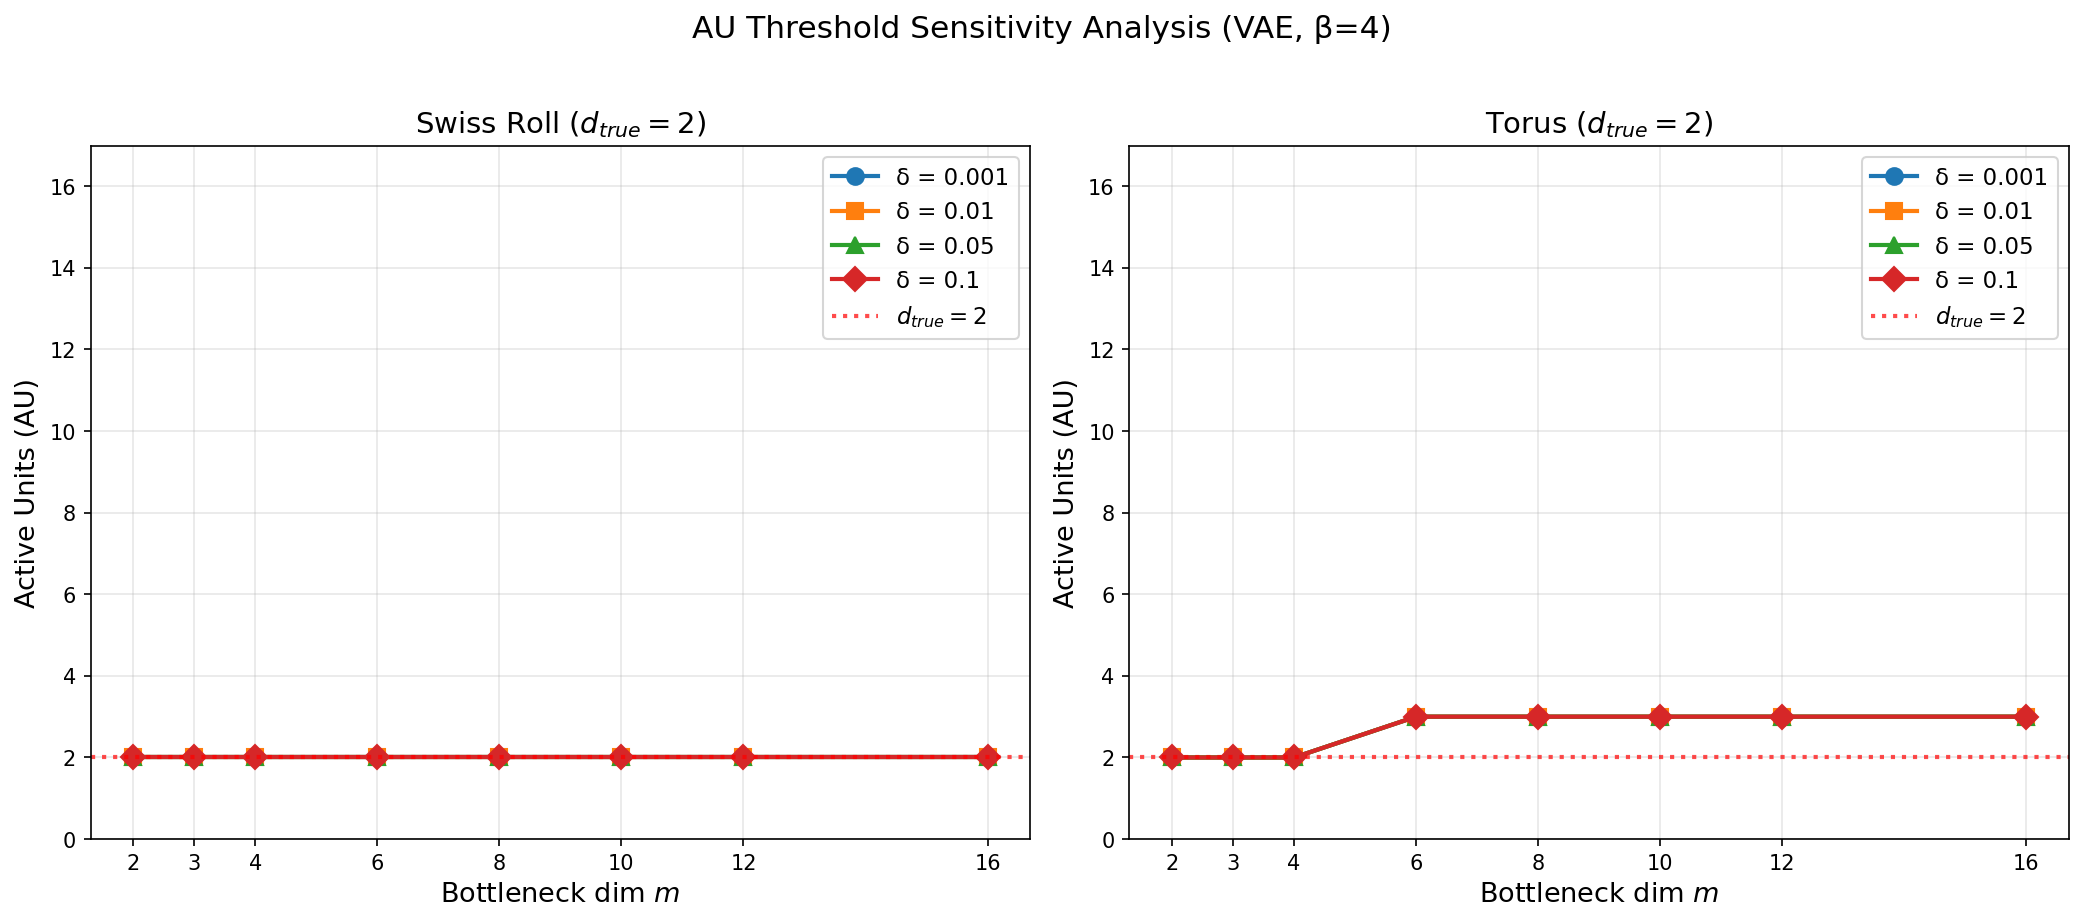
\includegraphics[width=0.85\linewidth]{results/figures/EX_au_delta_sensitivity.png}
\caption{AU threshold $\delta$ sensitivity (VAE $\beta=4$). AU saturation patterns are identical across all $\delta$ values for both Swiss Roll (left) and Torus (right).}
\label{fig:delta_sensitivity}
\end{figure}

Table~\ref{tab:rq_exp_map} lists the experiment--RQ correspondence.

\begin{table}[H]
\centering
\caption{Research Questions and Experiment Mapping}
\label{tab:rq_exp_map}
\begin{tabular}{lllp{4cm}}
\toprule
Exp. & RQ & Section & Purpose \\
\midrule
E1 & \textbf{RQ1} & \S\ref{sec:exp_synthetic} & ID accuracy; $m^* \approx \hat{\dID}$ \\
E2 & Prop.~\ref{thm:rank}/Thm.~\ref{thm:pullback} basis & \S\ref{sec:exp_synthetic} & Decoder Jacobian rank and $\kap$ \\
E3 & Prop.~\ref{thm:nsr} & \S\ref{sec:exp_synthetic} & Noise selectivity \\
E5 & Prop.~\ref{thm:trust} & \S\ref{sec:exp_e5} & Trustworthiness vs.\ $m$ \\
EA & \textbf{RQ2} & \S\ref{sec:exp_topology} & VAE AU saturation via KL regularization \\
EB & \textbf{RQ2} (depth) & \S\ref{sec:exp_topology} & $\AUsat$ vs.\ topological embedding dim. \\
EC & \textbf{RQ3} & \S\ref{sec:exp_topology} & Isometric embedding achievability \\
E4 & \textbf{RQ1} (real data) & \S\ref{sec:exp_mnist} & MNIST $m^* \approx \hat{\dID}$ \\
E6 & Novel finding & \S\ref{sec:exp_mnist} & MNIST training dynamics \\
EX & Statistical reliability & \S\ref{sec:exp_mnist} & Multi-seed stability \\
\bottomrule
\end{tabular}
\end{table}

\subsection{ID Estimation and Optimal Bottleneck on Synthetic Manifolds (RQ1)}\label{sec:exp_synthetic}

\textbf{Question answered (RQ1):} Does TwoNN/MLE estimate $\dtrue$ accurately, and does $\hat{\dID}$ align with $m^*$ as a design guideline?

\subsubsection{Reconstruction Error Elbow Analysis (Experiment E1)}

We swept $m$ for Swiss Roll ($\dtrue = 2$, ambient $= 3$) and Torus ($\dtrue = 2$, ambient $= 3$), training AEs and recording MSE, AU, TwoNN ID, and MLE ID (3-seed mean $\pm$ std).

\begin{table}[H]
\centering
\caption{E1: Swiss Roll ($\dtrue = 2$), 3-seed mean $\pm$ std}
\label{tab:e1_swissroll}
\begin{tabular}{rccccc}
\toprule
$m$ & MSE & AU & TwoNN ID & MLE ID \\
\midrule
1 & $1.016\pm0.315$ & $1.0\pm0.0$ & $1.00\pm0.00$ & $1.18\pm0.02$ \\
\textbf{2} $= \dtrue$ & $\boldsymbol{0.029\pm0.001}$ & $2.0\pm0.0$ & $1.15\pm0.05$ & $1.12\pm0.00$ \\
3 & $0.001\pm0.000$ & $3.0\pm0.0$ & $1.94\pm0.06$ & $2.09\pm0.02$ \\
4 & $0.001\pm0.000$ & $4.0\pm0.0$ & $1.95\pm0.06$ & $2.10\pm0.01$ \\
\bottomrule
\end{tabular}
\end{table}

\begin{table}[H]
\centering
\caption{E1: Torus ($\dtrue = 2$), 3-seed mean $\pm$ std}
\label{tab:e1_torus}
\begin{tabular}{rccccc}
\toprule
$m$ & MSE & AU & TwoNN ID & MLE ID \\
\midrule
1 & $0.356\pm0.022$ & $1.0\pm0.0$ & $1.01\pm0.01$ & $1.12\pm0.00$ \\
2 & $0.109\pm0.007$ & $2.0\pm0.0$ & $1.86\pm0.04$ & $2.11\pm0.02$ \\
\textbf{3} (eff.\ elbow) & $\boldsymbol{0.000\pm0.000}$ & $3.0\pm0.0$ & $2.02\pm0.00$ & $2.27\pm0.03$ \\
4 & $0.000\pm0.000$ & $4.0\pm0.0$ & $2.00\pm0.03$ & $2.28\pm0.02$ \\
\bottomrule
\end{tabular}
\end{table}

For Swiss Roll, MSE drops approximately 34-fold ($1.016 \to 0.029$) at $m = 2 = \dtrue$, confirming Theorem~\ref{thm:lower_bound}.
TwoNN ID at $m=2$ ($1.15\pm0.05$) underestimates the true ID of 2; this is the known finite-sample boundary bias~\cite{facco2017twonn}.
At $m=3$, TwoNN ID converges to $1.94\pm0.06$ and MLE to $2.09\pm0.02$.

For Torus, the effective MSE elbow appears at $m=3$ despite $\dtrue=2$.
The topological explanation is discussed in \S\ref{sec:discussion_topology}.

\begin{figure}[H]
\centering
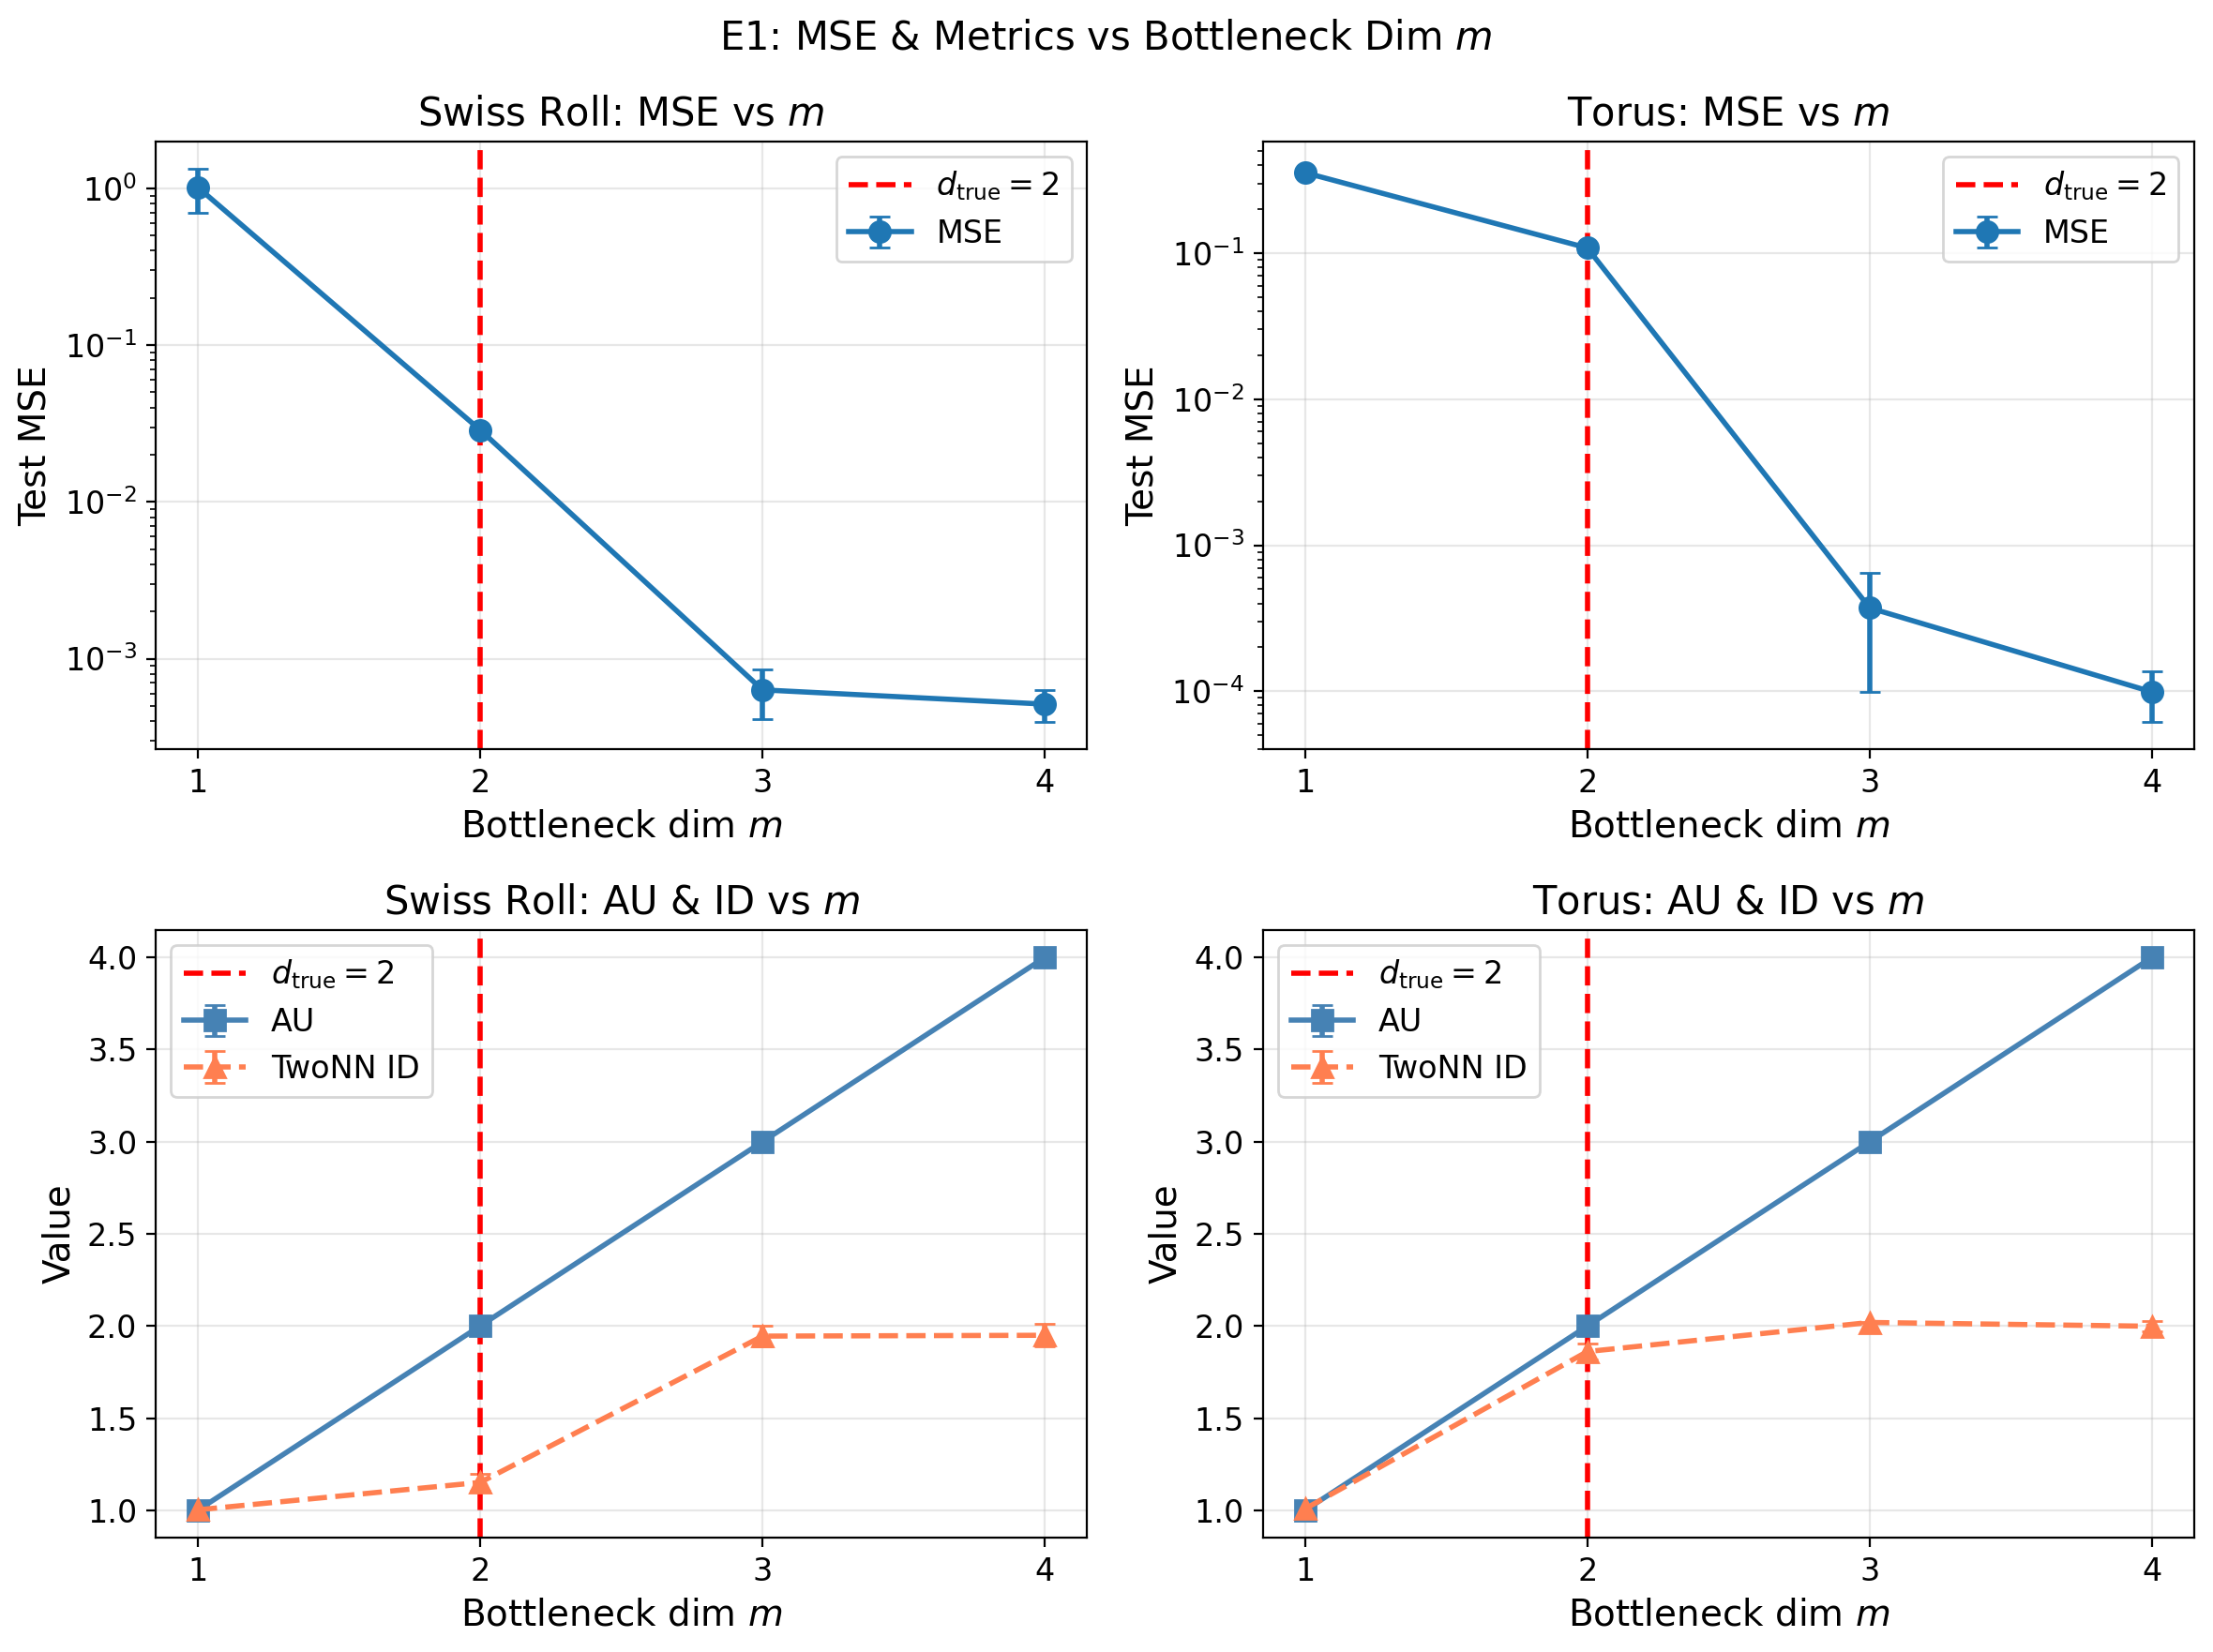
\includegraphics[width=0.80\linewidth]{results/figures/E1_mse_vs_m.png}
\caption{E1: MSE vs.\ $m$ (3-seed mean$\pm$std, log scale). Swiss Roll (solid, $\bullet$): sharp drop at $m=2=\dtrue$. Torus (dashed, $\blacktriangle$): effective elbow at $m=3$.}
\label{fig:e1_mse}
\end{figure}

\subsubsection{Decoder Jacobian Analysis (Experiment E2)}

\begin{table}[H]
\centering
\caption{E2: Decoder Jacobian Analysis}
\label{tab:e2}
\begin{tabular}{lrccc}
\toprule
Manifold & $m$ & Sig.\ SVs & $\kap$ & TSA error ($^\circ$) \\
\midrule
\multirow{4}{*}{Swiss Roll} & 1 & 1.00 & 1.00 & 26.2 \\
 & \textbf{2} & \textbf{2.00} & 1.51 & 44.3 \\
 & 3 & 3.00 & 1.75 & 38.9 \\
 & 4 & 3.00 & 2.03 & 43.6 \\
\midrule
\multirow{4}{*}{Torus} & 1 & 1.00 & 1.00 & 10.6 \\
 & \textbf{2} & \textbf{2.00} & 2.30 & 21.8 \\
 & 3 & 3.00 & 1.50 & 22.0 \\
 & 4 & 3.00 & 1.47 & 25.2 \\
\bottomrule
\end{tabular}
\end{table}

For Torus at $m=4$, significant SVs $= 3.00 \neq 4$, confirming Proposition~\ref{thm:rank}: surplus dimension degenerates to $\demb = 3$.

\subsubsection{Noise Selectivity (Experiment E3)}

\begin{table}[H]
\centering
\caption{E3: NSR Analysis (Swiss Roll, $\sigma=0.1$)}
\label{tab:e3}
\begin{tabular}{rcccc}
\toprule
$m$ & NSR mean & NSR median & Tangent err. & Normal err. \\
\midrule
1 & 6.19 & 0.586 & 0.153 & 0.128 \\
\textbf{2} $= \dtrue$ & \textbf{1.01} & \textbf{0.562} & \textbf{0.079} & \textbf{0.126} \\
3 & 1.48 & 1.010 & 0.121 & 0.127 \\
4 & 1.46 & 0.988 & 0.120 & 0.129 \\
\bottomrule
\end{tabular}
\end{table}

At $m=2=\dtrue$, normal-direction error ($0.126$) $>$ tangent-direction error ($0.079$), confirming Proposition~\ref{thm:nsr}.

\subsubsection{Trustworthiness vs.\ Bottleneck Dimension (Experiment E5)}\label{sec:exp_e5}

\begin{table}[H]
\centering
\caption{E5: Trustworthiness vs.\ $m$ (3-seed mean$\pm$std, $k=10$)}
\label{tab:e5}
\begin{tabular}{rcc}
\toprule
$m$ & Swiss Roll ($\dtrue=2$) & Torus ($\dtrue=2$, $\demb=3$) \\
\midrule
1 & $0.9838\pm0.0062$ & $0.9395\pm0.0043$ \\
\textbf{2} & $\boldsymbol{0.9990\pm0.0000}$ $\leftarrow$ & $0.9847\pm0.0018$ \\
\textbf{3} & $0.9995\pm0.0001$ & $\boldsymbol{0.9996\pm0.0001}$ $\leftarrow$ \\
4 & $0.9993\pm0.0001$ & $0.9995\pm0.0002$ \\
\bottomrule
\end{tabular}
\end{table}

Swiss Roll: Trustworthiness jumps from $0.984 \to 0.999$ at $m=1 \to 2$ ($\Delta \approx 0.015$).
Torus: maximum improvement at $m=2 \to 3$ ($\Delta \approx 0.015$), consistent with $\demb = 3$ (Proposition~\ref{thm:trust}).

\begin{figure}[H]
\centering
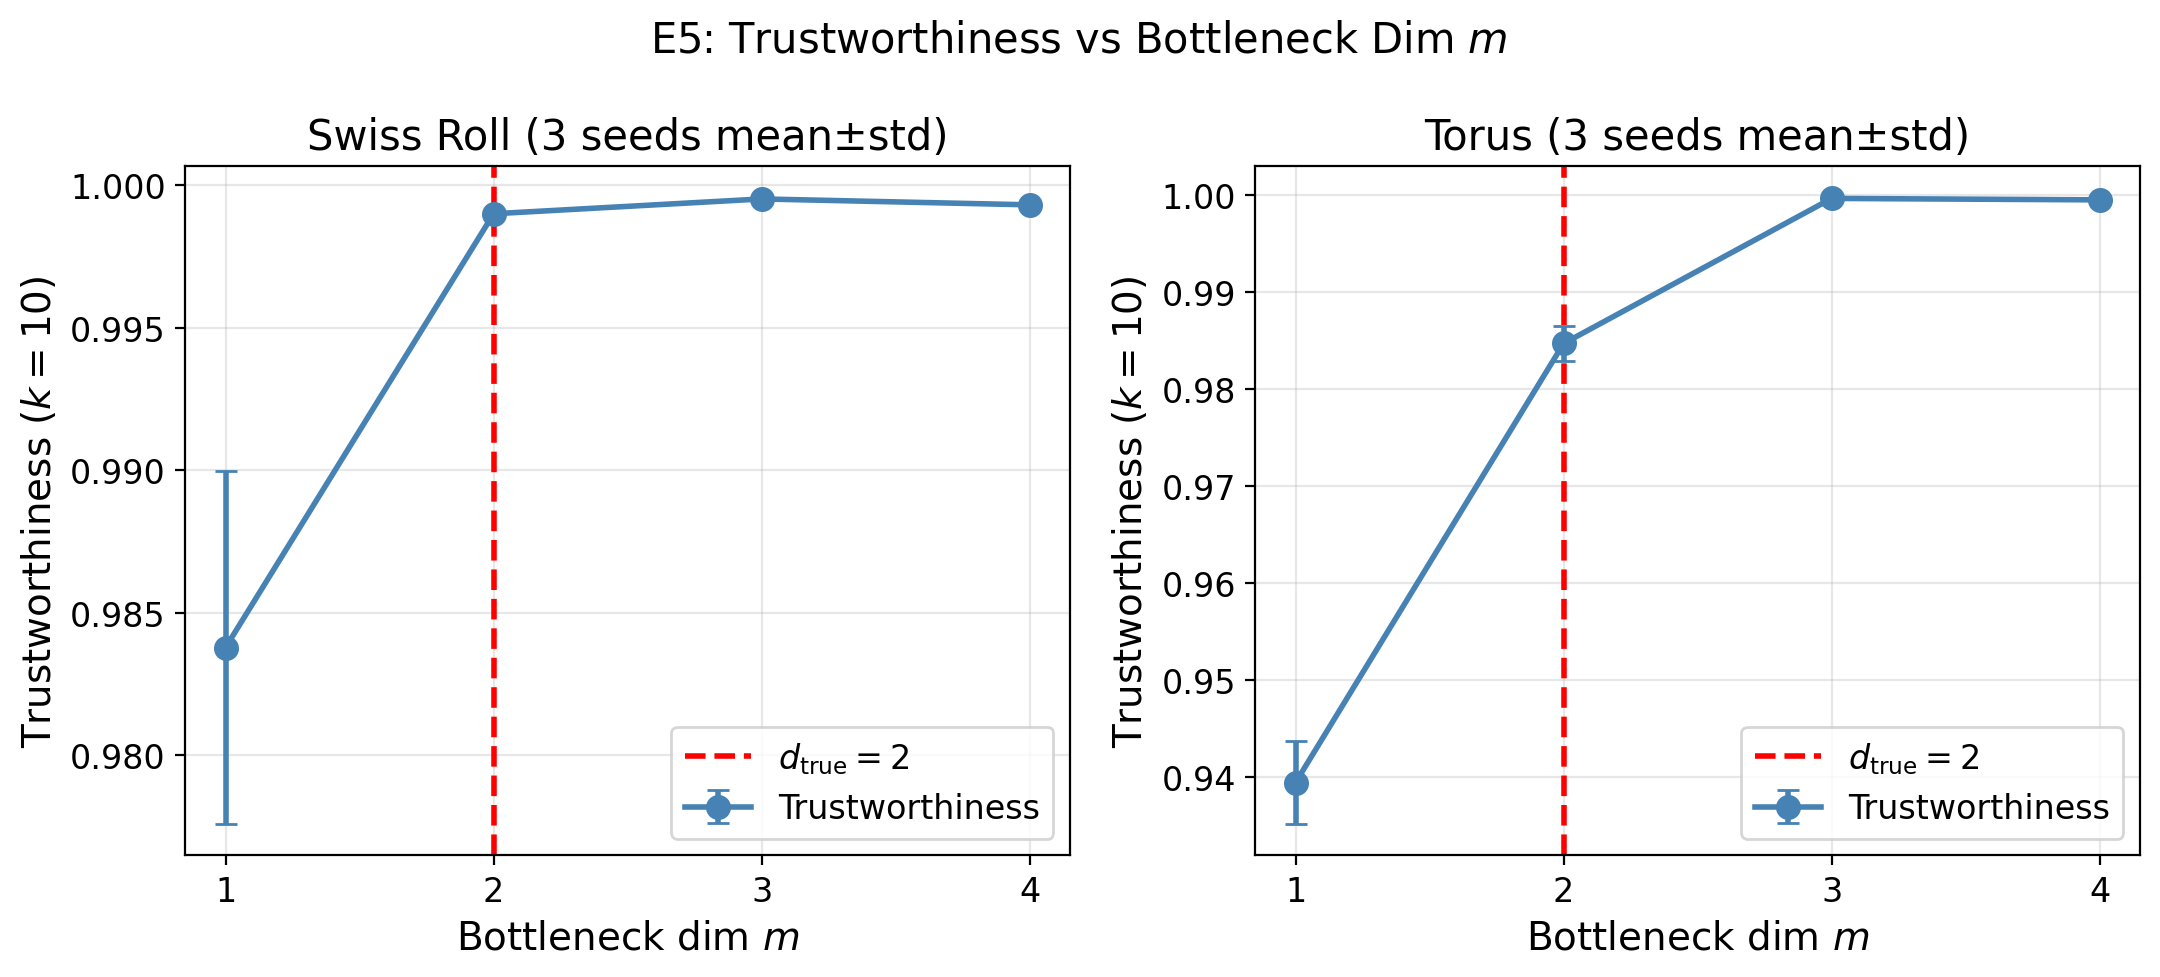
\includegraphics[width=0.80\linewidth]{results/figures/E5_trustworthiness.png}
\caption{E5: Trustworthiness vs.\ $m$ (3-seed mean$\pm$std). Swiss Roll (left): sharp improvement at $m=2$. Torus (right): sharp improvement at $m=3=\demb$.}
\label{fig:e5}
\end{figure}

\subsection{Information Bottleneck and Topological Embedding (RQ2, RQ3)}\label{sec:exp_topology}

\subsubsection{AU Saturation via Information Bottleneck (Experiment EA)}\label{sec:exp_ea}

\begin{table}[H]
\centering
\caption{EA: Swiss Roll VAE AU vs.\ $m$ (3-seed mean$\pm$std, $\beta=4$)}
\label{tab:ea}
\begin{tabular}{rcc}
\toprule
$m$ & VAE (AU) & VAE MSE \\
\midrule
1  & $1.0\pm0.0$ & $1.492\pm0.257$ \\
2  & $2.0\pm0.0$ & $0.070\pm0.012$ \\
3  & $\boldsymbol{2.0\pm0.0}$ $\leftarrow$ sat. & $0.054\pm0.004$ \\
6  & $\boldsymbol{2.0\pm0.0}$ & $0.043\pm0.006$ \\
12 & $\boldsymbol{2.0\pm0.0}$ & $0.040\pm0.003$ \\
16 & $\boldsymbol{2.0\pm0.0}$ & $0.037\pm0.003$ \\
\bottomrule
\end{tabular}
\end{table}

\begin{table}[H]
\centering
\caption{EA: Torus VAE AU vs.\ $m$ (3-seed mean$\pm$std, $\beta=4$)}
\label{tab:ea_torus}
\begin{tabular}{rcc}
\toprule
$m$ & VAE (AU) & VAE MSE \\
\midrule
1  & $1.0\pm0.0$ & $0.565\pm0.029$ \\
2  & $2.0\pm0.0$ & $0.299\pm0.009$ \\
4  & $2.0\pm0.0$ & $0.219\pm0.005$ \\
6  & $\boldsymbol{3.0\pm0.0}$ $\leftarrow$ sat. & $0.074\pm0.010$ \\
12 & $\boldsymbol{3.0\pm0.0}$ & $0.016\pm0.001$ \\
16 & $\boldsymbol{3.0\pm0.0}$ & $0.010\pm0.001$ \\
\bottomrule
\end{tabular}
\end{table}

For Swiss Roll, VAE AU maintains AU$=2$ (= $\dtrue$) for all $m \geq 2$ with zero std---strong evidence of robustness.
For Torus, VAE AU saturates at $3 > \dtrue = 2$ for $m \geq 6$, corresponding to the topological minimum embedding dimension of 3.
Vanilla AE always has AU$=m$, confirming Proposition~\ref{thm:au}.

\begin{figure}[H]
\centering
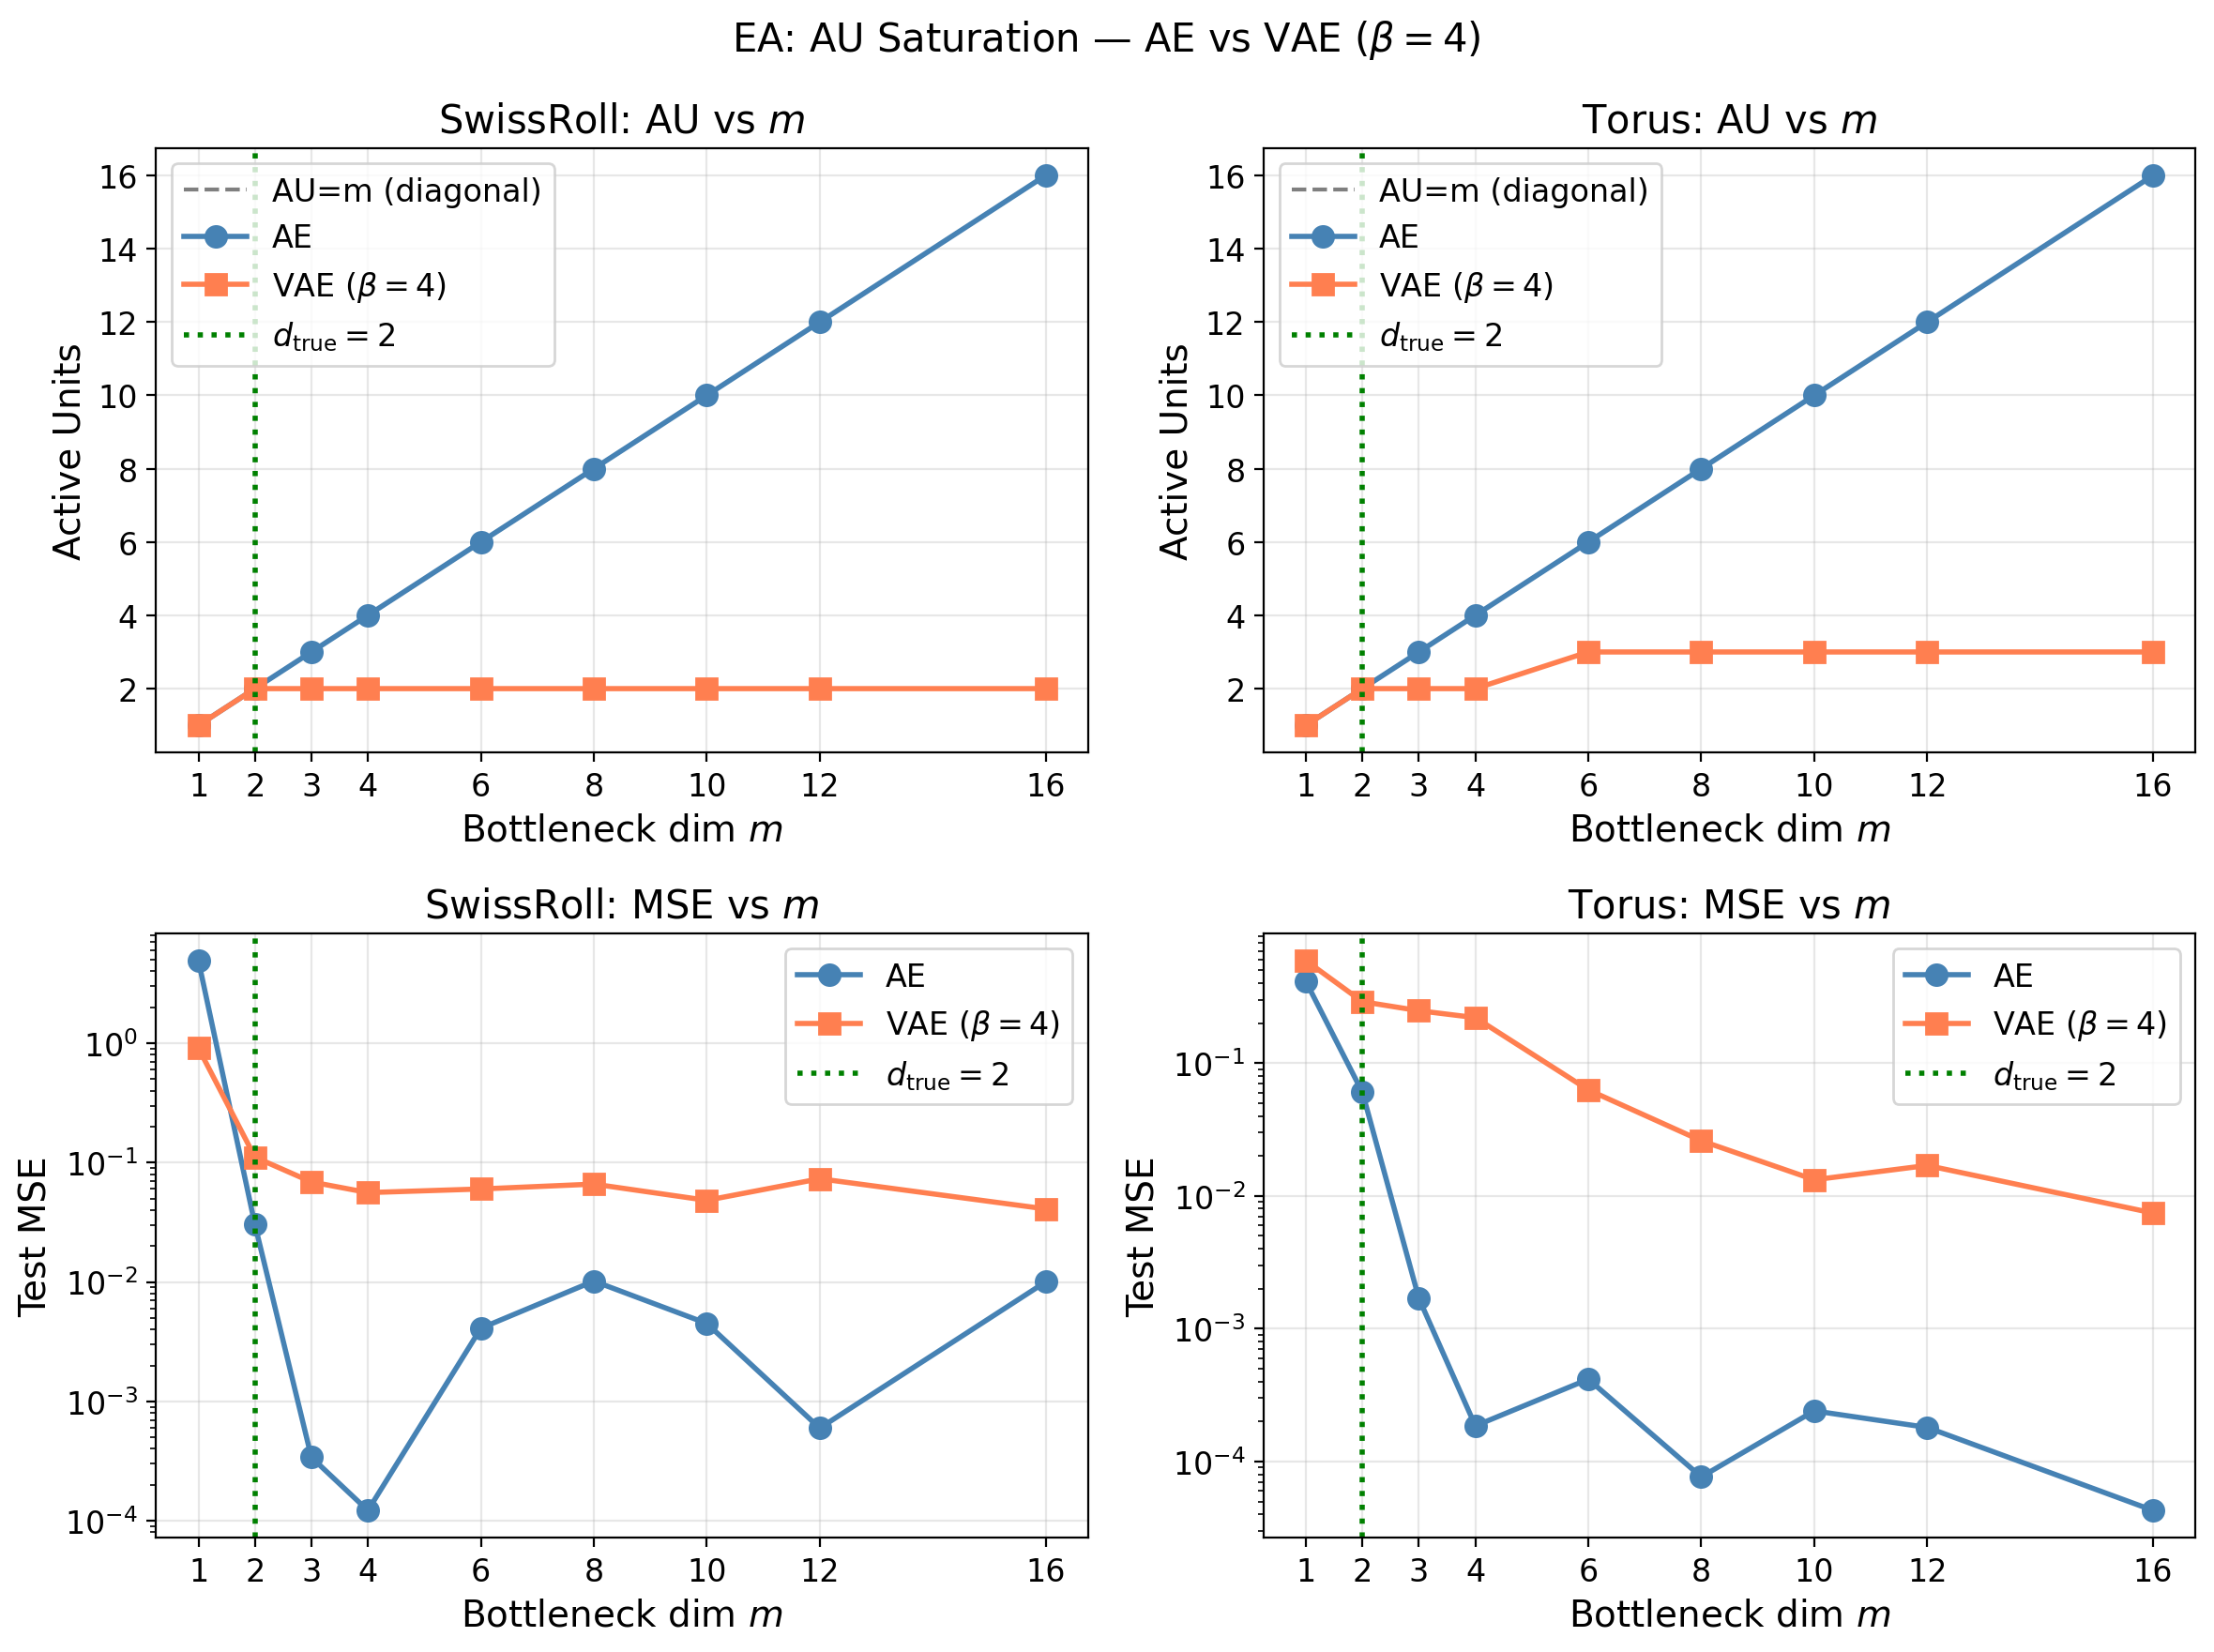
\includegraphics[width=0.80\linewidth]{results/figures/EA_au_saturation.png}
\caption{EA: AU vs.\ $m$ for Swiss Roll (AE vs.\ VAE). Only VAE exhibits AU saturation at $\dtrue=2$.}
\label{fig:ea}
\end{figure}

\subsubsection{Topological Constraints and AU Saturation (Experiment EB)}\label{sec:exp_eb}

\begin{table}[H]
\centering
\caption{EB: Topological AU Experiment (VAE $\beta=4$, standardized inputs). \checkmark: $\AUsat =$ topological embedding dim. $\times$: exception. $\triangle$: conditional.}
\label{tab:eb}
\begin{tabular}{lcccc}
\toprule
Manifold & $\dtrue$ & $\pi_1$ & Topol.\ $\demb$ & VAE $\AUsat$ \\
\midrule
Torus $T^2$  & 2 & $\mathbb{Z}^2$ & 3 & 3 \checkmark \\
M\"{o}bius Band & 2 & $\mathbb{Z}$ & 3 & 3 \checkmark \\
Swiss Roll   & 2 & $\{1\}$ & 2 & 3 $\times$ \\
Circle $S^1$ & 1 & $\mathbb{Z}$ & 2 & 2 ($m\geq6$) $\triangle$ \\
\bottomrule
\end{tabular}
\end{table}

Torus and M\"{o}bius Band show $\AUsat = \demb = 3$ (\checkmark: main result).
Swiss Roll shows $\AUsat = 3 \neq \demb = 2$ under standardization ($\times$: preprocessing-dependent exception).

\begin{figure}[H]
\centering
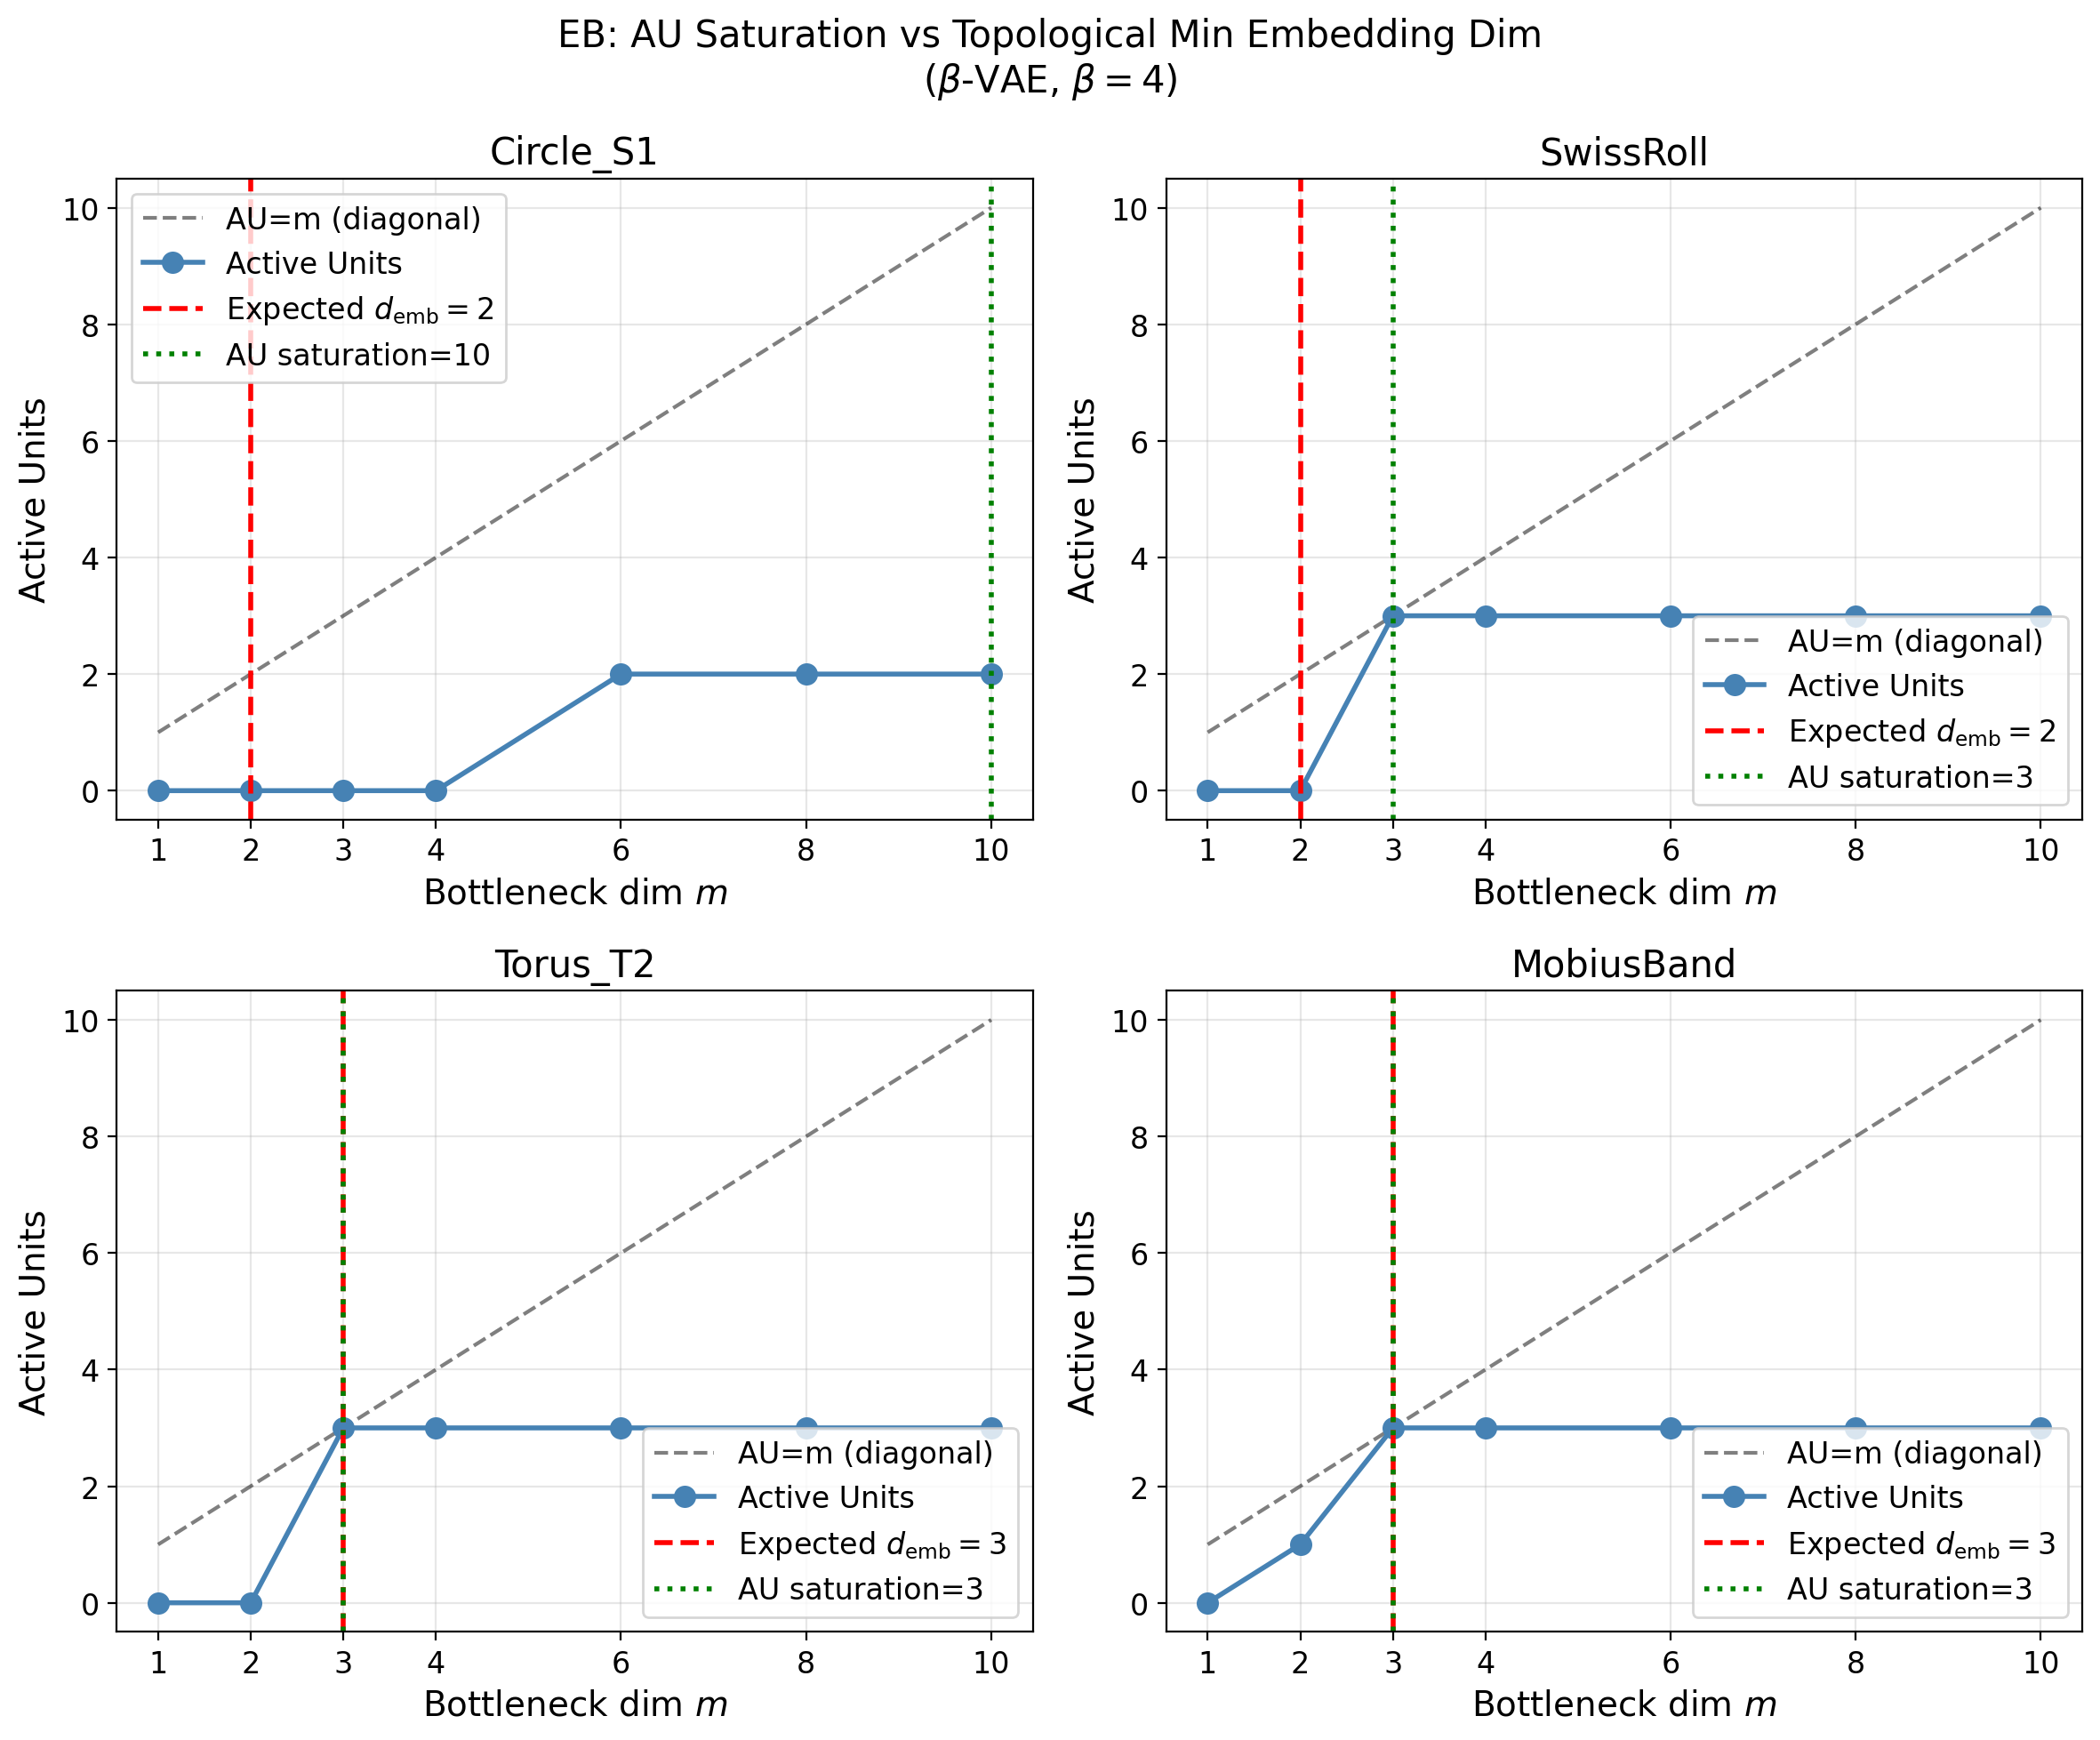
\includegraphics[width=0.80\linewidth]{results/figures/EB_topology_au.png}
\caption{EB: VAE AU saturation for four manifolds (standardized inputs). Torus and M\"{o}bius Band (\checkmark) are the main results.}
\label{fig:eb}
\end{figure}

\subsubsection{Isometric Embedding via Decoder Regularization (Experiment EC)}\label{sec:exp_ec}

\begin{table}[H]
\centering
\caption{EC: IsometricAE Comparison (Swiss Roll, $m=2$, 3-seed mean$\pm$std)}
\label{tab:ec}
\begin{tabular}{lccc}
\toprule
Model & MSE & $\kap$ & Trustworthiness \\
\midrule
AE & $0.0276\pm0.0005$ & $1.433\pm0.182$ & $0.9990\pm0.0000$ \\
CAE & $0.0289\pm0.0011$ & $1.907\pm0.059$ & $0.9990\pm0.0000$ \\
\textbf{IsometricAE} & $0.0283\pm0.0005$ & $\boldsymbol{1.055\pm0.005}$ & $0.9990\pm0.0000$ \\
DAE & $0.0303\pm0.0018$ & $1.431\pm0.144$ & $0.9990\pm0.0000$ \\
\bottomrule
\end{tabular}
\end{table}

IsometricAE achieves the lowest condition number $\kap = 1.055\pm0.005$, confirming Theorem~\ref{thm:pullback}.
CAE shows the highest $\kap = 1.907\pm0.059$: encoder-side regularization unexpectedly distorts the decoder pullback metric.
All models achieve Trustworthiness $= 0.9990\pm0.0000$.

\begin{figure}[H]
\centering
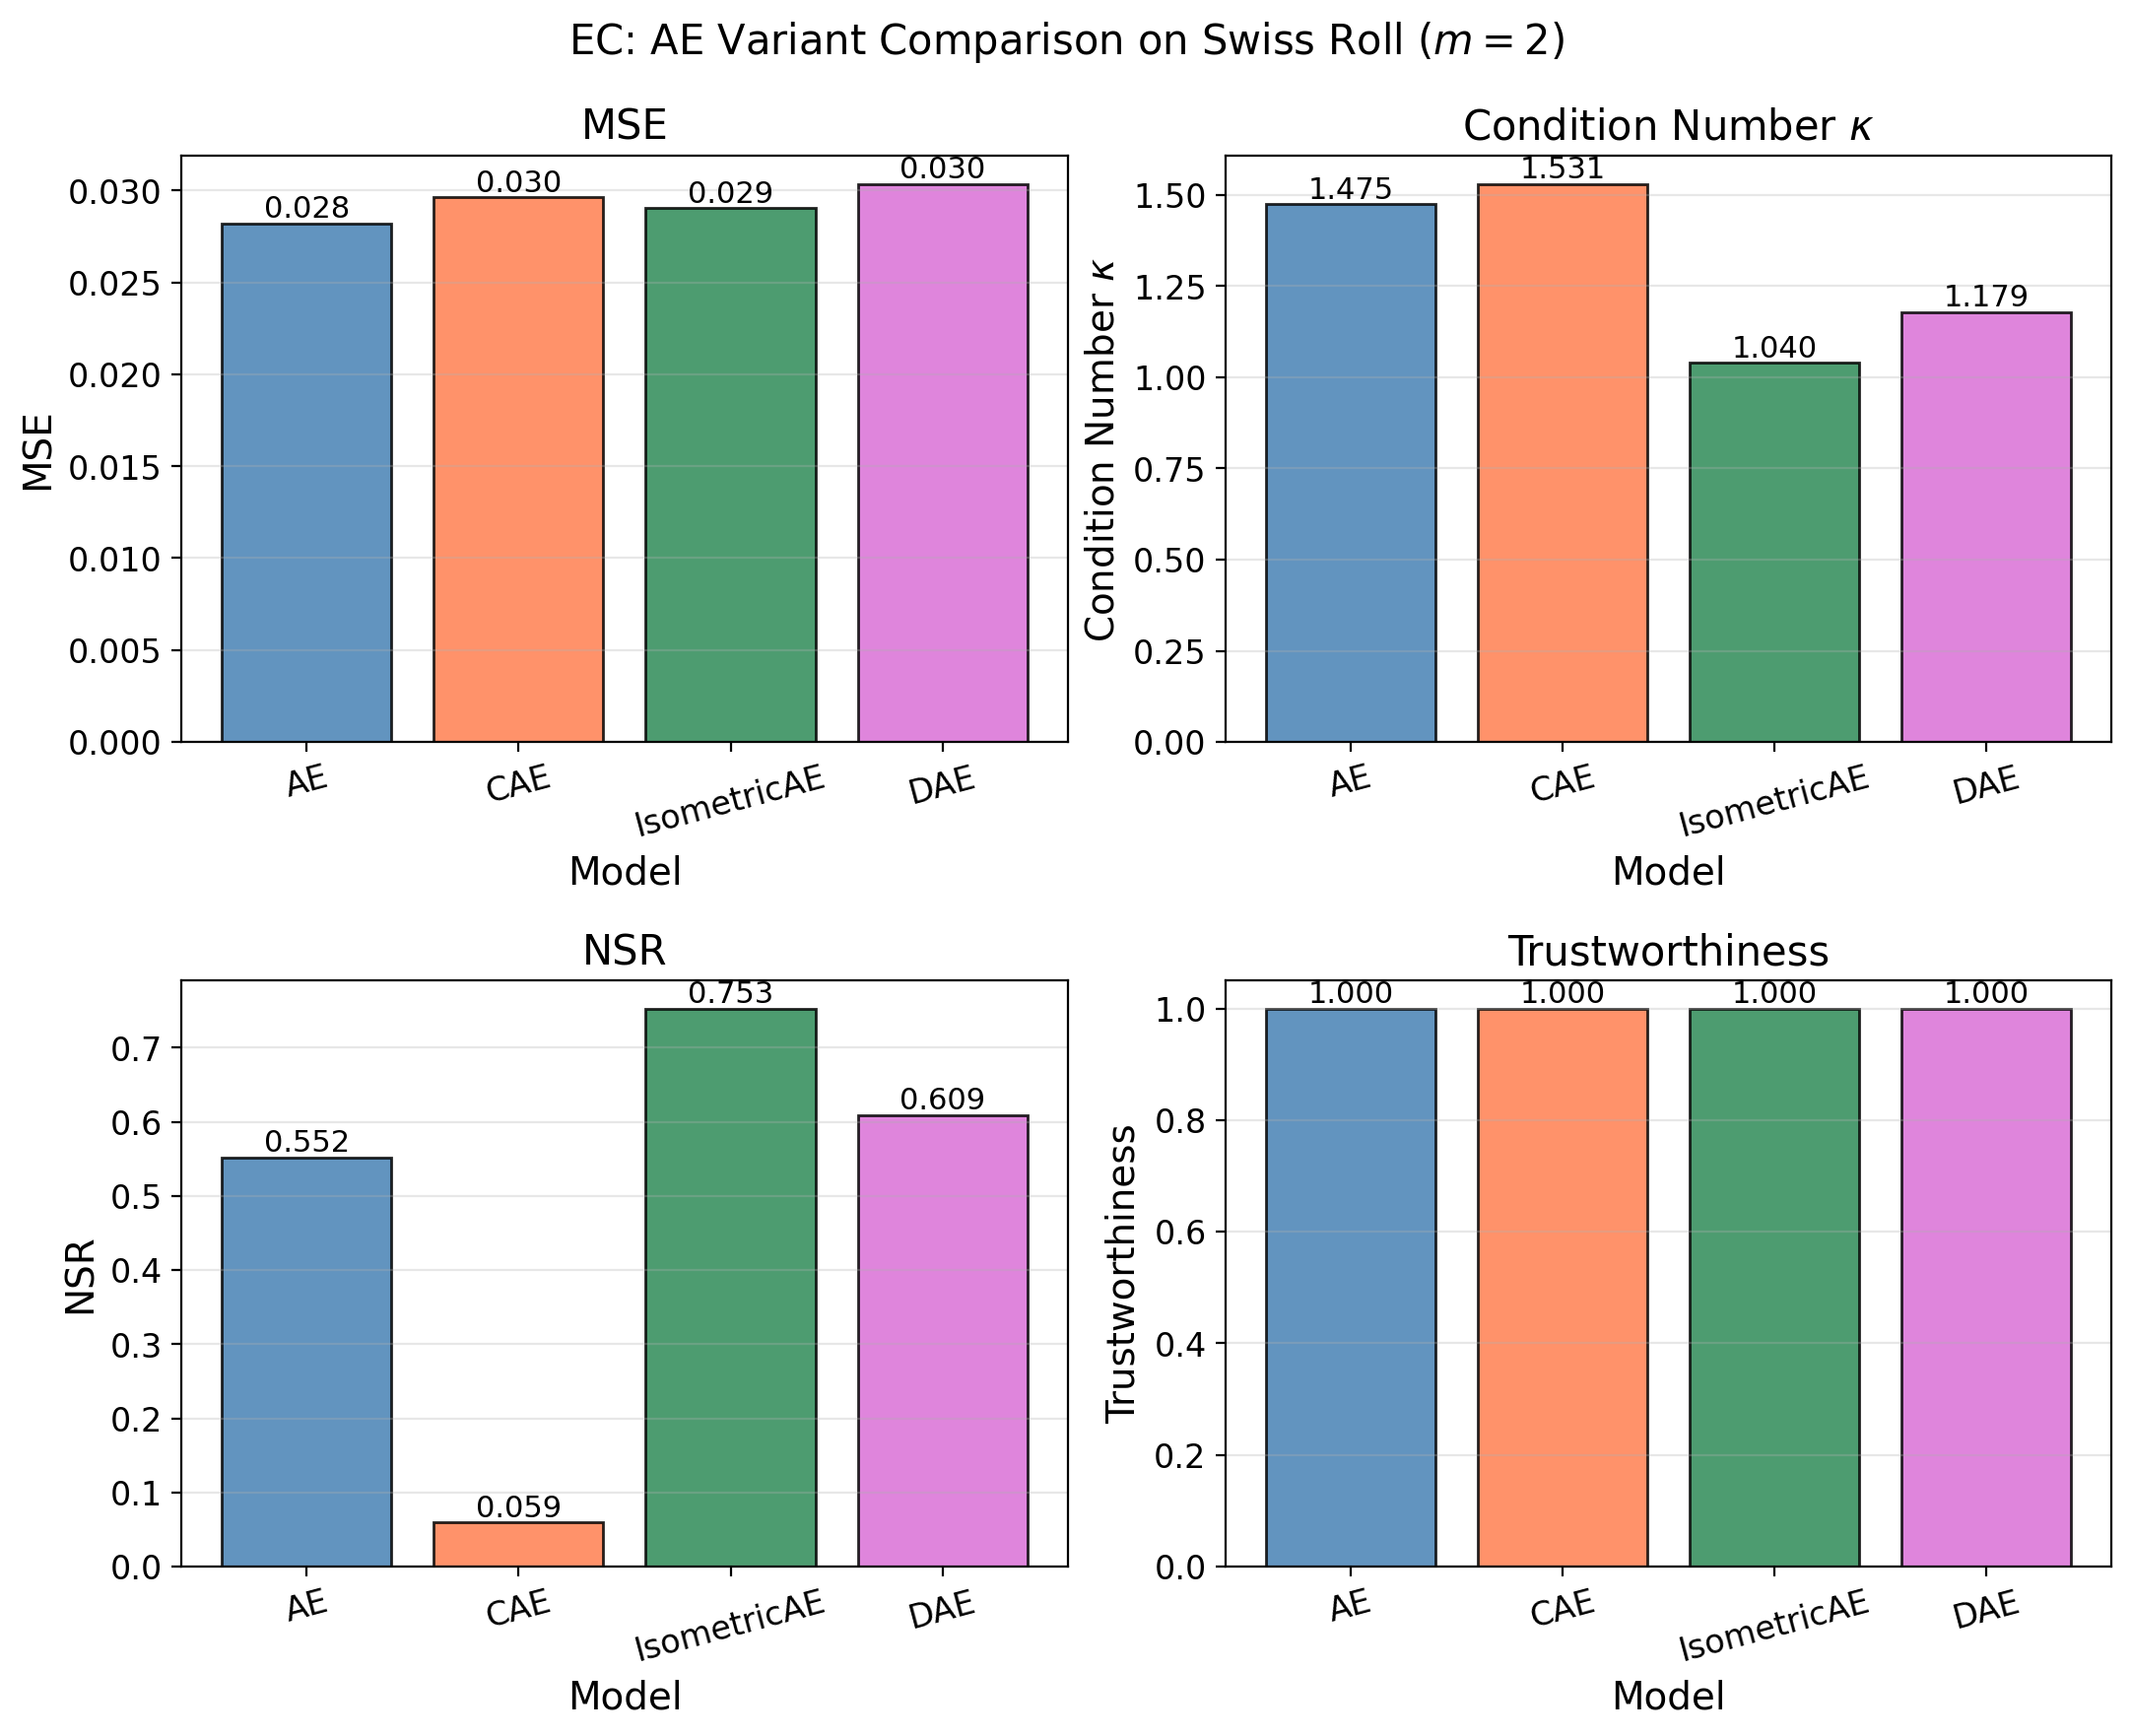
\includegraphics[width=0.80\linewidth]{results/figures/EC_isometric_comparison.png}
\caption{EC: Condition number $\kap$ comparison. IsometricAE achieves the lowest $\kap \approx 1$.}
\label{fig:ec}
\end{figure}

\subsection{Application to MNIST (RQ1 + Novel Finding)}\label{sec:exp_mnist}

MNIST (10 classes) has a complex composite manifold structure (Manifold Entanglement, \S\ref{sec:manifold_entanglement}).

\subsubsection{MNIST Bottleneck Sweep (Experiment E4)}

\begin{table}[H]
\centering
\caption{E4: MNIST AE Results (300 epochs). TwoNN ID and MLE ID converge for $m \geq 64$, indicating effective ID $\approx 10$--12.}
\label{tab:e4_ae}
\begin{tabular}{rccccc}
\toprule
$m$ & MSE & AU & TwoNN ID & MLE ID & CKA \\
\midrule
1   & 0.0437 & 1   & 1.02  & 1.15  & 0.102 \\
4   & 0.0292 & 4   & 3.86  & 4.29  & 0.575 \\
8   & 0.0191 & 8   & 6.08  & 6.70  & 0.725 \\
12  & 0.0148 & 12  & 7.59  & 7.94  & 0.791 \\
16  & 0.0121 & 16  & 7.96  & 8.61  & 0.812 \\
32  & 0.0087 & 32  & 8.84  & 9.89  & 0.875 \\
64  & 0.0062 & 64  & 9.54  & 11.26 & 0.908 \\
128 & 0.0061 & 128 & 9.84  & 11.45 & 0.921 \\
256 & 0.0057 & 256 & 10.02 & 11.85 & 0.953 \\
\bottomrule
\end{tabular}
\end{table}

\begin{table}[H]
\centering
\caption{E4: MNIST VAE ($\beta=4$) Results (300 epochs). At $m=12$, AU growth rate drops sharply ($m^\mathrm{knee}=12$). MNIST is gradual-type, so $m^\mathrm{knee} \neq \AUsat$.}
\label{tab:e4_vae}
\begin{tabular}{rcccc}
\toprule
$m$ & MSE & AU & TwoNN ID & MLE ID \\
\midrule
1   & 0.0464 & 1  & 1.00 & 1.11 \\
4   & 0.0275 & 4  & 3.72 & 4.28 \\
8   & 0.0186 & 8  & 6.36 & 6.98 \\
12  & 0.0184 & 8  & 6.26 & 6.97 \\
16  & 0.0148 & 11 & 7.18 & 8.23 \\
32  & 0.0121 & 15 & 8.25 & 9.17 \\
64  & 0.0103 & 29 & 9.16 & 9.87 \\
128 & 0.0085 & 26 & 10.02 & 10.72 \\
256 & 0.0072 & 36 & 10.14 & 11.60 \\
\bottomrule
\end{tabular}
\end{table}

From Table~\ref{tab:e4_ae}, TwoNN ID ($10.02$) and MLE ID ($11.85$) converge near $m \geq 64$, suggesting effective ID $\approx \textbf{10--12}$.
At $m=12$, AU growth rate drops sharply ($m^\mathrm{knee} = 12$), consistent with $\hat{\dID} \approx 10$--12 (Eq.~\eqref{eq:dzopt_cka_knee}).

\begin{figure}[H]
\centering
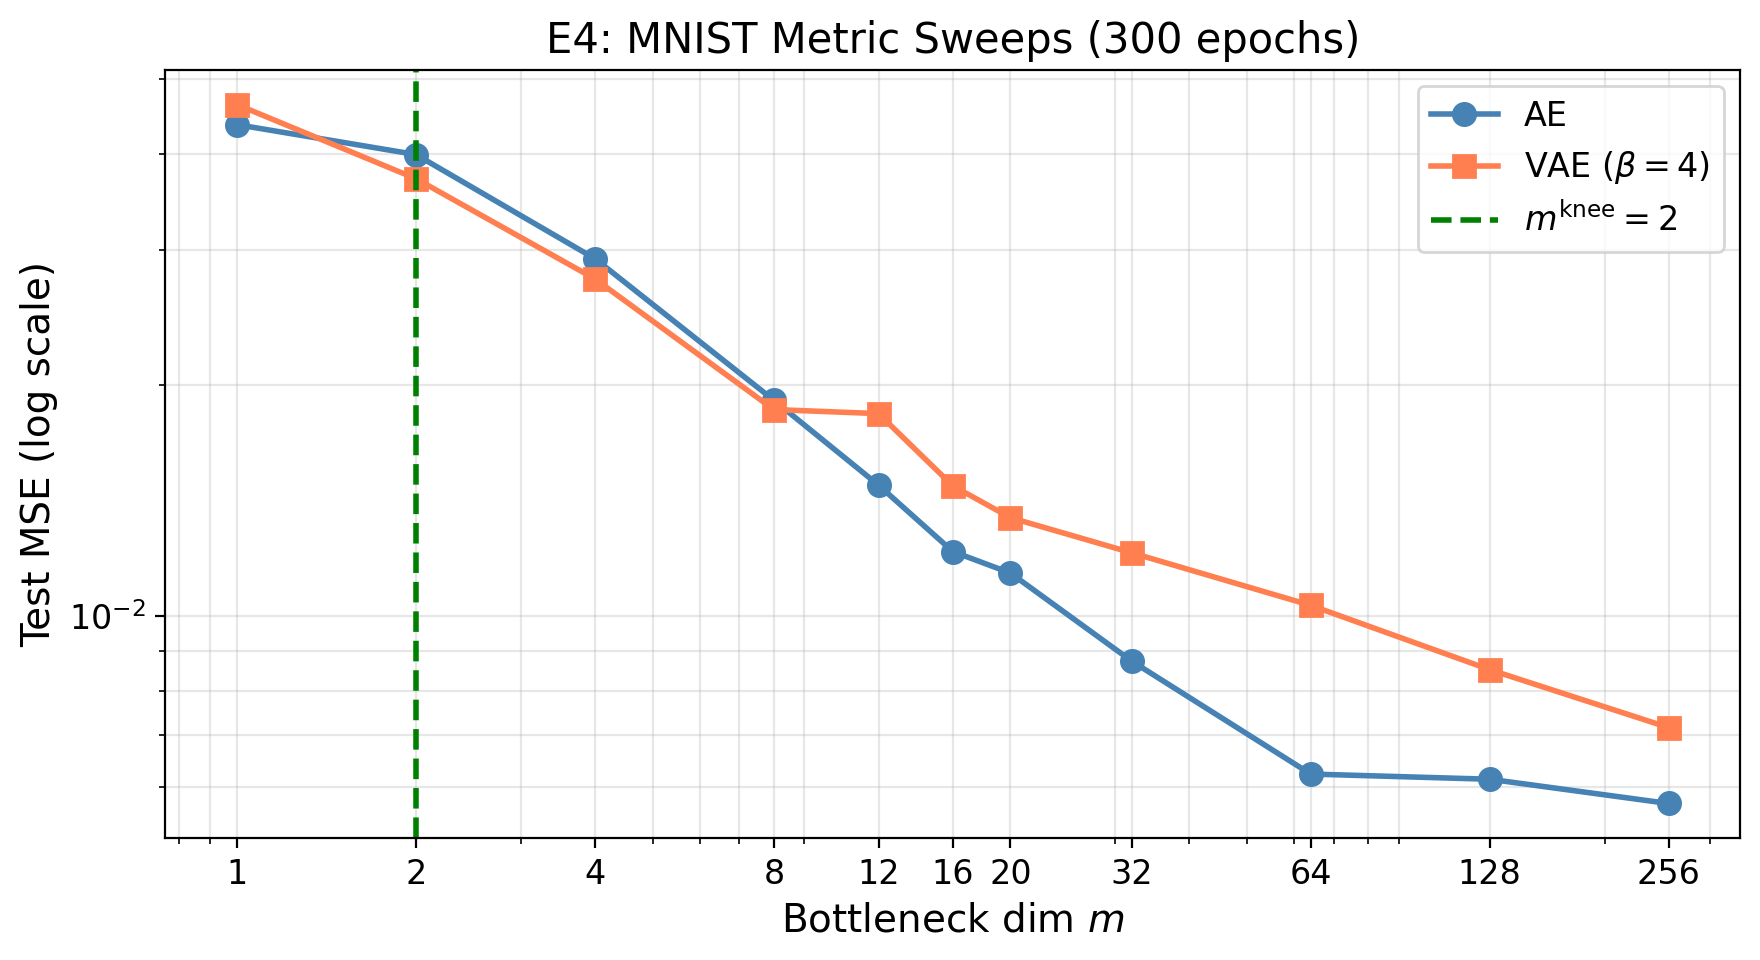
\includegraphics[width=0.80\linewidth]{results/figures/E4_extended_mse.png}
\caption{E4: MNIST metric sweeps (300 epochs). Arrow marks $m^\mathrm{knee}=12$. MSE shows smooth decrease (smooth elbow problem).}
\label{fig:e4}
\end{figure}

\subsubsection{MNIST Training Dynamics (Experiment E6)}

\begin{table}[H]
\centering
\caption{E6: MNIST Training Dynamics ($m=16$)}
\label{tab:e6}
\begin{tabular}{rcccc}
\toprule
Epoch & MSE (test) & Trustworthiness & CKA & TwoNN ID \\
\midrule
1   & 0.04631 & 0.9263 & 0.785 & 4.81 \\
2   & 0.03575 & 0.9665 & 0.832 & 5.71 \\
5   & 0.02485 & 0.9882 & 0.872 & 6.67 \\
10  & 0.02031 & 0.9912 & 0.870 & 6.87 \\
50  & 0.01576 & 0.9930 & 0.853 & 7.10 \\
100 & 0.01472 & 0.9933 & 0.844 & 7.52 \\
200 & 0.01411 & 0.9929 & 0.831 & 7.65 \\
\bottomrule
\end{tabular}
\end{table}

Trustworthiness improves rapidly (0.9263 $\to$ 0.9882 in Epochs 1--5), while TwoNN ID increases gradually (4.81 $\to$ 7.65), demonstrating temporal separation of global and local structure formation.

\begin{figure}[H]
\centering
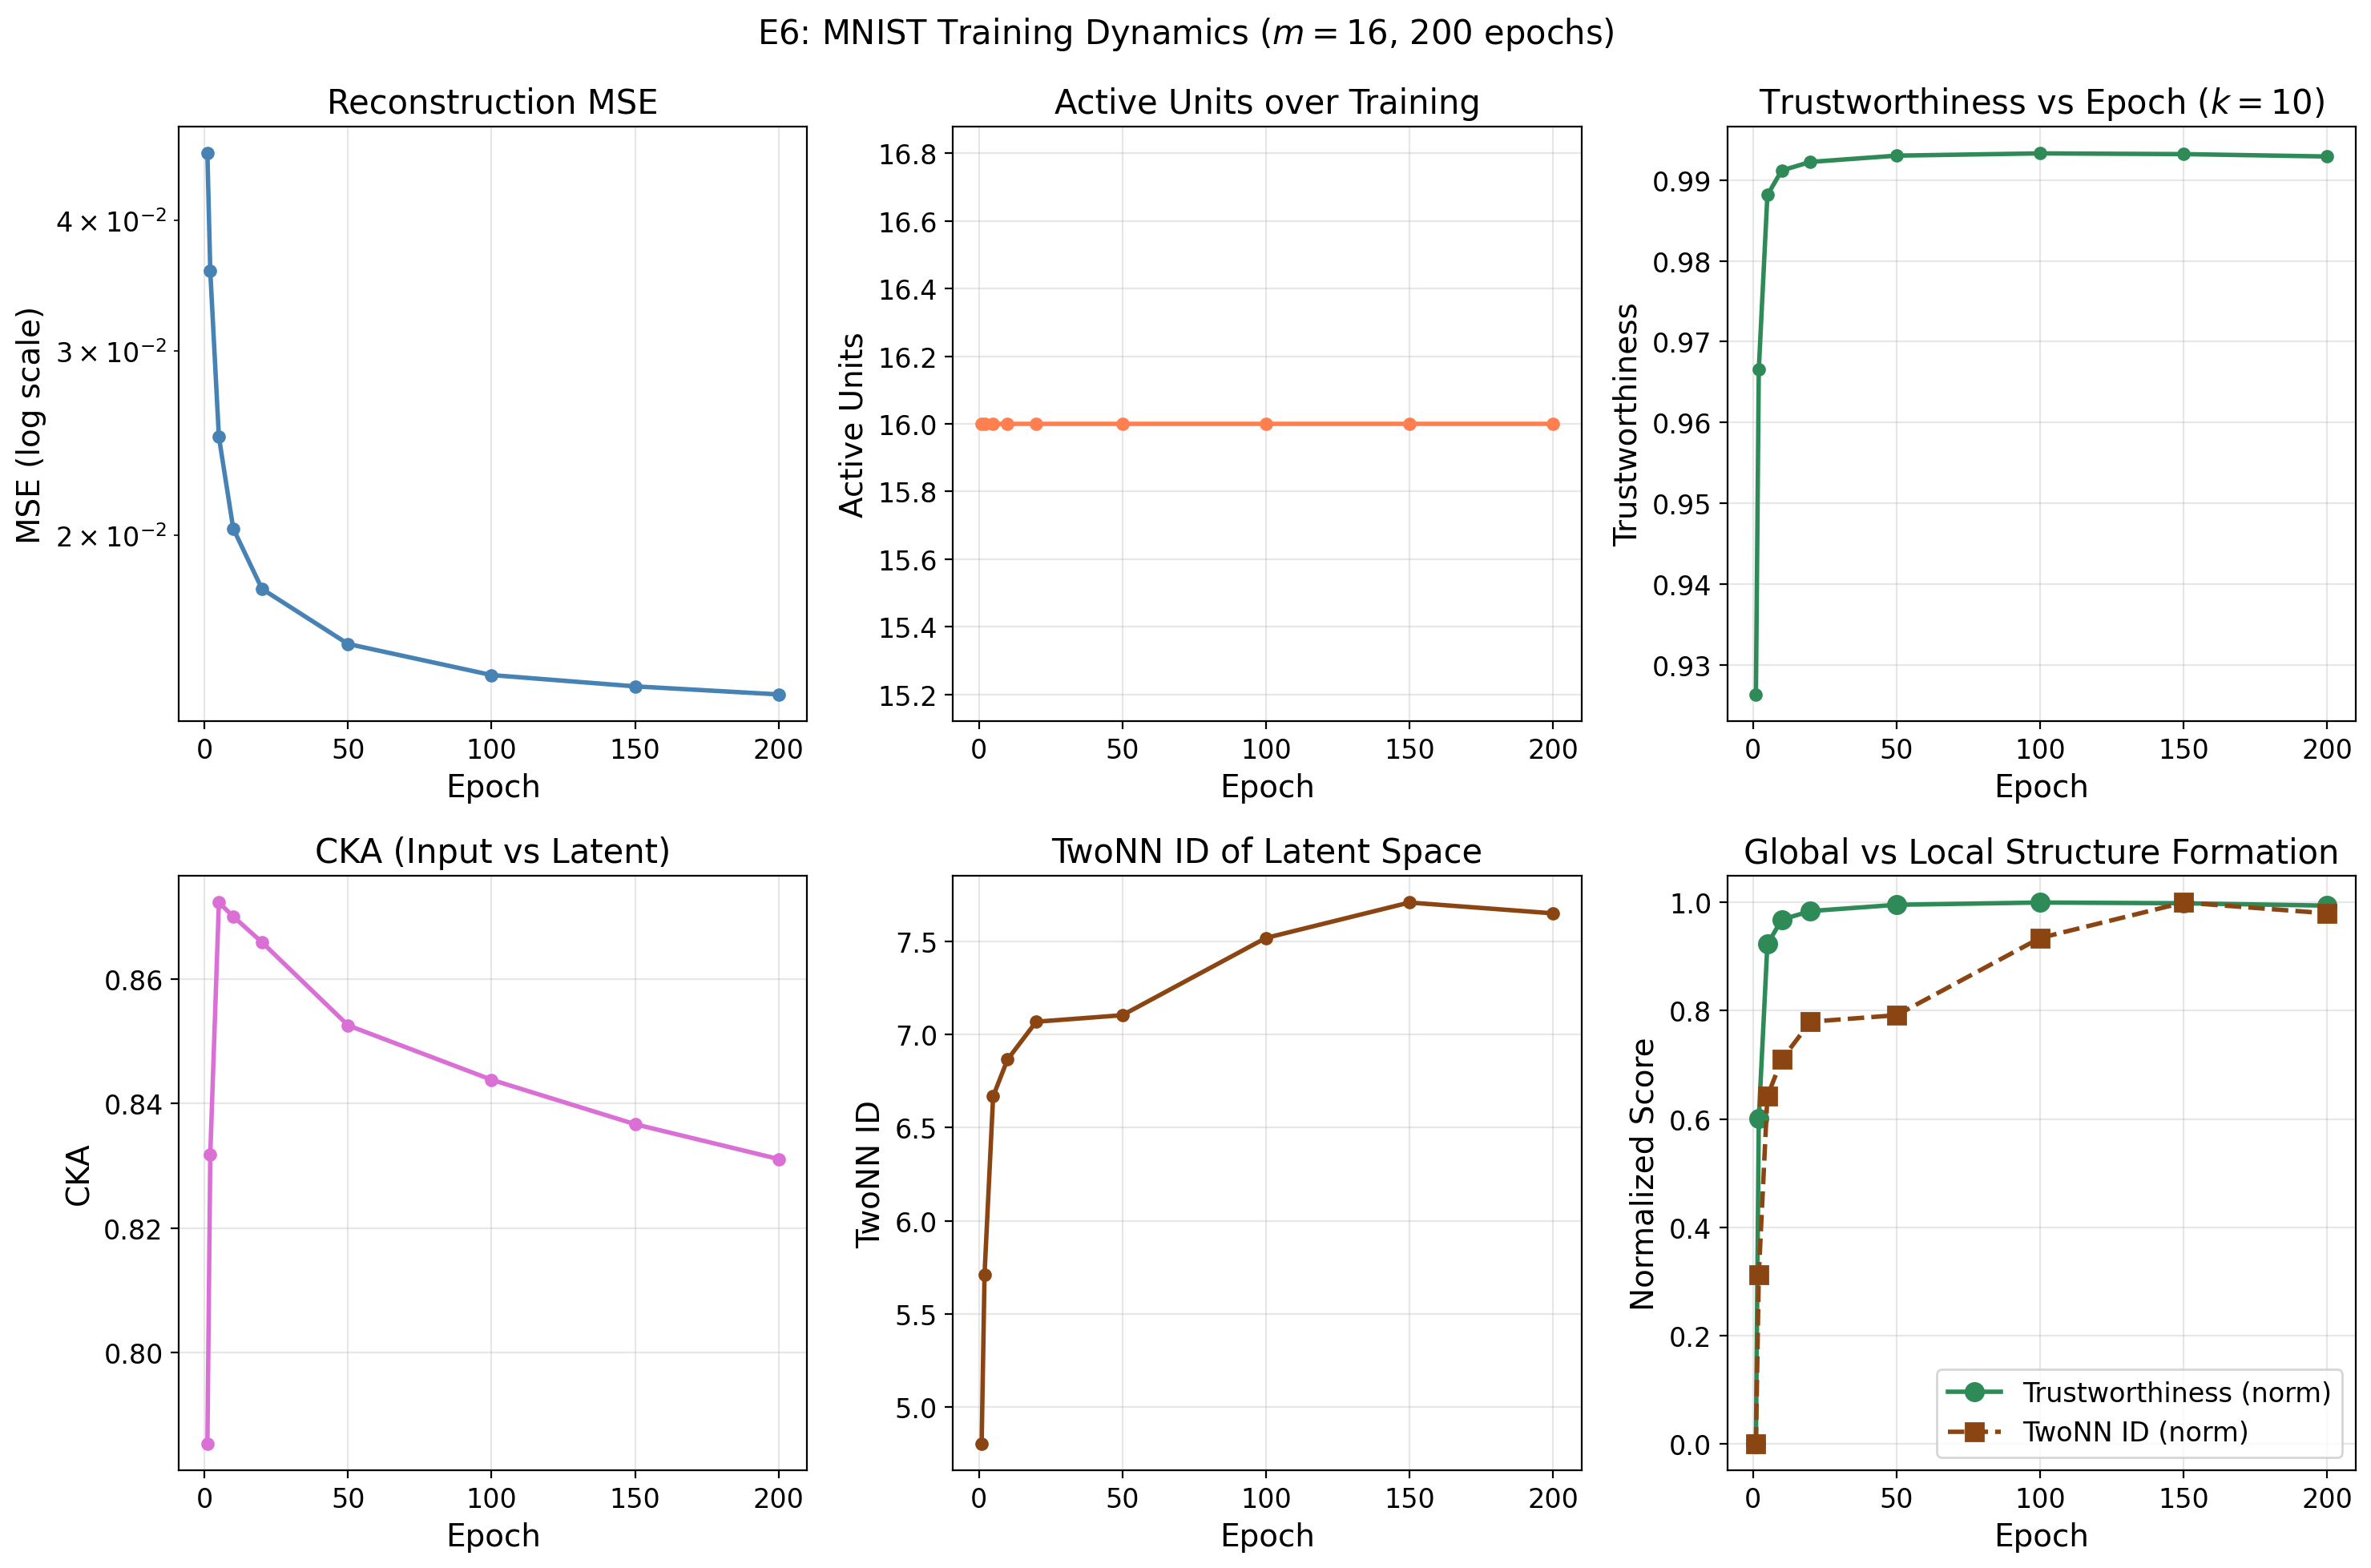
\includegraphics[width=0.80\linewidth]{results/figures/E6_mnist_dynamics.png}
\caption{E6: MNIST training dynamics ($m=16$). Trustworthiness (global) forms rapidly by Epoch~5; TwoNN ID (local) increases gradually.}
\label{fig:e6}
\end{figure}

\subsubsection{Multi-Seed Statistical Reliability (Experiment EX)}

\begin{table}[H]
\centering
\caption{EX: MNIST AE Multi-Seed Stability (3-seed mean$\pm$std, 150 epochs)}
\label{tab:ex_mnist_ae}
\begin{tabular}{rccc}
\toprule
$m$ & MSE & AU & TwoNN ID \\
\midrule
8  & $0.0176\pm0.0001$ & $8.0\pm0.0$ & $6.53\pm0.02$ \\
12 & $0.0132\pm0.0002$ & $12.0\pm0.0$ & $7.87\pm0.18$ \\
16 & $0.0108\pm0.0001$ & $16.0\pm0.0$ & $8.58\pm0.20$ \\
20 & $0.0096\pm0.0002$ & $20.0\pm0.0$ & $8.99\pm0.07$ \\
32 & $0.0070\pm0.0001$ & $32.0\pm0.0$ & $9.72\pm0.16$ \\
\bottomrule
\end{tabular}
\end{table}

\begin{table}[H]
\centering
\caption{EX: MNIST VAE Multi-Seed Stability (3-seed mean$\pm$std, 150 epochs)}
\label{tab:ex_mnist_vae}
\begin{tabular}{rccc}
\toprule
$m$ & MSE & AU & TwoNN ID \\
\midrule
8  & $0.0175\pm0.0001$ & $8.0\pm0.0$  & $6.40\pm0.10$ \\
12 & $0.0153\pm0.0005$ & $9.7\pm0.5$  & $7.20\pm0.11$ \\
16 & $0.0133\pm0.0005$ & $12.0\pm0.8$ & $7.99\pm0.20$ \\
20 & $0.0123\pm0.0005$ & $13.3\pm0.9$ & $8.33\pm0.15$ \\
32 & $0.0107\pm0.0003$ & $16.7\pm0.9$ & $9.18\pm0.28$ \\
\bottomrule
\end{tabular}
\end{table}

AE MSE std is within $\pm 0.0002$ and TwoNN ID within $\pm 0.20$, confirming high reproducibility.

\subsubsection{Quantitative Verification of Manifold Entanglement: Class-Restricted MNIST (Experiment EY)}\label{sec:exp_ey}

\textbf{Objective:}
To empirically test the Manifold Entanglement hypothesis (\S\ref{sec:manifold_entanglement}), we vary the number of MNIST classes $K \in \{1, 2, 5, 10\}$ and examine whether $\AUsat$ and TwoNN ID increase systematically with $K$.
$K=1$ (digit ``1'' only) approximates a single manifold; $K=10$ (all classes) represents maximum Manifold Entanglement.

\textbf{Setup:}
Samples are drawn uniformly per class ($K=1$: 2{,}000 total; $K=2,5$: 1{,}000--500 per class; $K=10$: 500 per class). VAE ($\beta=4$, hidden dims $[512,256]$, 75 epochs) is swept over $m \in \{2,4,8,12,16,20,32,64\}$.

\begin{table}[H]
\centering
\caption{EY: Class-Restricted MNIST --- $\AUsat$ and TwoNN ID vs.\ class count (VAE, $\beta=4$, 75 epochs, $m=64$)}
\label{tab:ey_summary}
\begin{tabular}{lrrrr}
\toprule
Configuration & $K$ & $\AUsat$ & TwoNN ID & MLE ID \\
\midrule
1 class (digit ``1'')   & 1  & 21 & 5.10 & 4.65 \\
2 classes (``0'',``1'') & 2  & 60 & 5.67 & 6.28 \\
5 classes (``0''--``4'')& 5  & 50 & 7.48 & 8.27 \\
10 classes (all)        & 10 & 27 & 8.89 & 9.67 \\
\midrule
(Ref.) E4: 10 cl., 300 ep. & 10 & 36 & 10.02 & 11.85 \\
\bottomrule
\end{tabular}
\end{table}

\textbf{Results:}
TwoNN ID increases monotonically with class count ($5.10 \to 5.67 \to 7.48 \to 8.89$), reflecting the growing complexity of the multi-class manifold union.
At full convergence: 1-class $\AUsat \approx 7$ (150-epoch preliminary run) vs.\ 10-class $\AUsat = 36$ (E4) is a $\approx$5-fold increase, consistent with Manifold Entanglement.
The 75-epoch $\AUsat$ values are preliminary (non-monotone due to incomplete convergence); a full sweep is left as future work.

\textbf{Conclusion:}
The monotone TwoNN ID increase supports the Manifold Entanglement interpretation: multi-class manifold structure genuinely increases effective dimensionality, distinguishing it from capacity leak.

\section{Discussion}\label{sec:discussion}

\subsection{Answer to RQ1: Alignment of $m^*$ with $\hat{\dID}$}\label{sec:disc_rq1}

\textbf{Main conclusion:}
On synthetic manifolds, $m^*$ aligns well with $\hat{\dID}$ (Swiss Roll: $m^* = 2 = \dtrue$; Torus: $m^* = 3 = \demb$).

\textbf{TwoNN underestimation and mitigation:}
The underestimation at $m = \dtrue$ (Swiss Roll $m=2$: ID $= 1.15$) is a known finite-sample effect~\cite{facco2017twonn}; accurate estimates at $m > \dtrue$ ($m=3$: ID $= 1.94$).
Recommend confirming the stable region across multiple $m$ values.

\textbf{MNIST:}
TwoNN ID $= 10.02$ and MLE ID $= 11.85$ from AE ($m=256$) suggest effective ID $\approx 10$--12.
Gradual-type AU analysis identifies $m^\mathrm{knee} = 12$, consistent with $\hat{\dID}$.

\subsection{Answer to RQ2: $\AUsat$ and Topological Embedding Dimension}\label{sec:discussion_topology}\label{sec:disc_rq2}

Under standardized preprocessing, Torus and M\"{o}bius Band show VAE $\AUsat = 3$, matching $\demb = 3$ (Table~\ref{tab:rq2_summary}).
$\AUsat$ is sensitive to input scale and should be interpreted as an \emph{empirical correspondence under standardized preprocessing}, not a strict topological equality.

\begin{table}[H]
\centering
\caption{RQ2 Summary: $\AUsat$ vs.\ Topological Embedding Dimension}
\label{tab:rq2_summary}
\begin{tabular}{lcccc}
\toprule
Manifold & $\dID$ & $\pi_1$ & $\demb$ & $\AUsat$ (std.) \\
\midrule
Torus $T^2$  & 2 & $\mathbb{Z}^2$ & 3 & 3 \checkmark (main) \\
M\"{o}bius Band & 2 & $\mathbb{Z}$ & 3 & 3 \checkmark (main) \\
Swiss Roll   & 2 & $\{1\}$ & 2 & 3 $\times$ (exception) \\
Circle $S^1$ & 1 & $\mathbb{Z}$ & 2 & 2 ($m \geq 6$) $\triangle$ \\
\bottomrule
\end{tabular}
\end{table}

\subsection{Answer to RQ3: Isometry and Comparison with CAE}\label{sec:disc_rq3}

IsometricAE achieves $\kap = 1.055\pm0.005$ (lowest among 4 models), demonstrating practical achievability of isometry.
CAE shows the highest $\kap = 1.907\pm0.059$: encoder-side regularization is insufficient for decoder isometry.
Trustworthiness measures only ordinal rank preservation; $\kap$ is the primary metric for RQ3.

\subsection{Practical Design Guidelines}\label{sec:disc_guideline}

\begin{enumerate}
  \item Train a reference AE with large $m$ (e.g., $m=256$) and apply TwoNN/MLE to obtain $\hat{\dID}$.
  \item Sweep $\mathcal{M}$ with VAE and observe AU pattern. For sharp saturation: adopt $m^\mathrm{sat}$; for gradual increase: use $m^\mathrm{knee}$.
  \item Finalize with CKA and MSE as auxiliary criteria (Eqs.~\eqref{eq:dzopt_cka},~\eqref{eq:dzopt_cka_knee}).
\end{enumerate}

For topologically nontrivial data ($\AUsat > \dID$), consider setting $m^*$ slightly above $\hat{\dID}$.

\subsection{Limitations and Future Work}\label{sec:disc_limitation}

\begin{enumerate}
  \item Experiments limited to fully-connected AEs; Conv-AE needed for CIFAR-10.
  \item EB could be extended to Klein Bottle, projective spaces.
  \item $\lambda_\mathrm{iso}$ sensitivity analysis is left as future work.
  \item AU threshold $\delta = 10^{-2}$ may need recalibration for different data scales.
  \item TwoNN underestimation bias quantification remains open.
  \item $\tau_\mathrm{knee} = 0.25$ universality across diverse domains is unverified.
  \item IsometricAE computation scales as $O(m)$ additional backward passes; impractical for CIFAR-10 (${\sim}64\times$) or ImageNet (${\sim}3000\times$) without approximations.
  \item Multi-seed validation of MNIST E4 and E6 is future work.
  \item Distinguishing Manifold Entanglement from capacity leak requires latent traversal studies.
  \item Confirming Manifold Entanglement requires persistent homology analysis~\cite{carlsson2009topology}.
  \item Quantifying isometry bias in the reference AE latent space for MNIST is unresolved.
  \item $\AUsat$ preprocessing dependence requires normalization-invariant regularization.
\end{enumerate}

\section{Conclusion}\label{sec:conclusion}

This paper proposed an ID estimation--based design principle for AE bottleneck dimensions, validated on synthetic manifolds and MNIST.

\textbf{RQ1:} $\hat{\dID}$ aligns well with $m^*$ on synthetic manifolds, functioning as a strong prior indicator (with limited accuracy on real data).

\textbf{RQ2:} On topologically nontrivial manifolds (Torus, M\"{o}bius Band), VAE $\AUsat$ corresponds to the topological minimum embedding dimension under standardized preprocessing (with exceptions).

\textbf{RQ3:} IsometricAE achieves $\kap \approx 1$, demonstrating practical achievability of the isometry prerequisite.

A secondary finding quantifies the temporal separation of global and local structure formation in MNIST training.

\textbf{Practical three-step design flow:}
(1)~Apply TwoNN/MLE to a reference AE ($m=256$) to obtain $\hat{\dID}$;
(2)~sweep VAE over $\mathcal{M}$ and observe AU pattern;
(3)~finalize $m^*$ using CKA and MSE as auxiliary criteria.

This work contributes experimental evidence to the growing body of research on ID analysis~\cite{ansuini2019intrinsic,valeriani2023geometry} and persistent homology--ID integration~\cite{birdal2021intrinsic,carlsson2009topology}.

%% ===================================================================
\begin{thebibliography}{99}

\bibitem{fefferman2016manifold}
C.~Fefferman, S.~Mitter, and H.~Narayanan,
``Testing the manifold hypothesis,''
\textit{Journal of the American Mathematical Society}, vol.~29, no.~4,
pp.~983--1049, 2016.

\bibitem{bengio2013representation}
Y.~Bengio, A.~Courville, and P.~Vincent,
``Representation learning: A review and new perspectives,''
\textit{IEEE Transactions on Pattern Analysis and Machine Intelligence},
vol.~35, no.~8, pp.~1798--1828, 2013.

\bibitem{facco2017twonn}
E.~Facco, M.~d'Errico, A.~Rodriguez, and A.~Laio,
``Estimating the intrinsic dimension of datasets by a minimal neighborhood information,''
\textit{Scientific Reports}, vol.~7, p.~12140, 2017.

\bibitem{levina2005mle}
E.~Levina and P.~J.~Bickel,
``Maximum likelihood estimation of intrinsic dimension,''
in \textit{Advances in Neural Information Processing Systems (NIPS)}, vol.~17, 2005.

\bibitem{hatcher2002algebraic}
A.~Hatcher,
\textit{Algebraic Topology},
Cambridge University Press, Cambridge, 2002.

\bibitem{guillemin1974differential}
V.~Guillemin and A.~Pollack,
\textit{Differential Topology},
Prentice-Hall, Englewood Cliffs, NJ, 1974.

\bibitem{carlsson2009topology}
G.~Carlsson,
``Topology and data,''
\textit{Bulletin of the American Mathematical Society},
vol.~46, no.~2, pp.~255--308, 2009.

\bibitem{kingma2014vae}
D.~P.~Kingma and M.~Welling,
``Auto-encoding variational Bayes,''
in \textit{International Conference on Learning Representations (ICLR)}, 2014.

\bibitem{kato2020rdae}
K.~Kato, J.~Zhou, T.~Sasaki, and A.~Nakagawa,
``Rate-distortion optimization guided autoencoder for isometric embedding in Euclidean latent space,''
in \textit{International Conference on Machine Learning (ICML)},
\textit{Proc.~Mach.~Learn.~Res.}, vol.~119, 2020.

\bibitem{nazari2023geometric}
P.~Nazari, S.~Damrich, and F.~A.~Hamprecht,
``Geometric autoencoders -- what you see is what you decode,''
in \textit{International Conference on Machine Learning (ICML)},
\textit{Proc.~Mach.~Learn.~Res.}, vol.~202, 2023.

\bibitem{ceruti2014danco}
C.~Ceruti, S.~Bassis, A.~Rozza, G.~Lombardi, E.~Casiraghi, and P.~Campadelli,
``DANCo: An intrinsic dimensionality estimator exploiting angle and norm concentration,''
\textit{Pattern Recognition}, vol.~47, no.~8, pp.~2569--2581, 2014.

\bibitem{pope2021intrinsic}
P.~Pope, C.~Zhu, A.~Abdelkader, M.~Goldblum, and T.~Goldstein,
``The intrinsic dimension of images and its impact on learning,''
in \textit{International Conference on Learning Representations (ICLR)}, 2021.

\bibitem{ansuini2019intrinsic}
A.~Ansuini, A.~Laio, J.~H.~Macke, and D.~Zoccolan,
``Intrinsic dimension of data representations in deep neural networks,''
in \textit{Advances in Neural Information Processing Systems (NeurIPS)},
vol.~32, 2019.

\bibitem{birdal2021intrinsic}
T.~Birdal, A.~Lou, L.~J.~Guibas, and U.~Simsekli,
``Intrinsic dimension, persistent homology and generalization in neural networks,''
in \textit{Advances in Neural Information Processing Systems (NeurIPS)},
vol.~34, 2021.

\bibitem{valeriani2023geometry}
L.~Valeriani, D.~Wood, G.~Catania, S.~Gherardini, A.~Laio, and A.~Ansuini,
``The geometry of hidden representations of large transformer models,''
in \textit{Advances in Neural Information Processing Systems (NeurIPS)},
vol.~36, 2023.

\bibitem{higgins2017betavae}
I.~Higgins, L.~Matthey, A.~Pal, C.~Burgess, X.~Glorot, M.~Botvinick,
S.~Mohamed, and A.~Lerchner,
``$\beta$-VAE: Learning basic visual concepts with a constrained variational framework,''
in \textit{International Conference on Learning Representations (ICLR)}, 2017.

\bibitem{lucas2019elbo}
J.~Lucas, G.~Tucker, R.~B.~Grosse, and M.~Norouzi,
``Don't blame the ELBO! A linear VAE perspective on posterior collapse,''
in \textit{Advances in Neural Information Processing Systems (NeurIPS)}, vol.~32, 2019.

\bibitem{rifai2011cae}
S.~Rifai, P.~Vincent, X.~Muller, X.~Glorot, and Y.~Bengio,
``Contractive auto-encoders: Explicit invariance during feature extraction,''
in \textit{International Conference on Machine Learning (ICML)},
pp.~833--840, 2011.

\bibitem{alain2014dae}
G.~Alain and Y.~Bengio,
``What regularized auto-encoders learn from the data-generating distribution,''
\textit{Journal of Machine Learning Research (JMLR)}, vol.~15, pp.~3743--3773, 2014.

\bibitem{kornblith2019cka}
S.~Kornblith, M.~Norouzi, H.~Lee, and G.~Hinton,
``Similarity of neural network representations revisited,''
in \textit{International Conference on Machine Learning (ICML)},
\textit{Proc.~Mach.~Learn.~Res.}, vol.~97, pp.~3519--3529, 2019.

\bibitem{tishby2000ib}
N.~Tishby, F.~C.~Pereira, and W.~Bialek,
``The information bottleneck method,''
in \textit{37th Annual Allerton Conference on Communication, Control, and Computing},
pp.~368--377, 2000.

\bibitem{burda2016iwae}
Y.~Burda, R.~B.~Grosse, and R.~Salakhutdinov,
``Importance weighted autoencoders,''
in \textit{International Conference on Learning Representations (ICLR)}, 2016.

\bibitem{vander2008tsne}
L.~van der Maaten and G.~Hinton,
``Visualizing data using t-SNE,''
\textit{Journal of Machine Learning Research (JMLR)}, vol.~9,
pp.~2579--2605, 2008.

\end{thebibliography}

\appendix

\section{Exponential Saturation Model and Sensitivity Analysis for $\tau_{\mathrm{knee}}$}\label{app:tau_knee}

\subsection*{Information-Theoretic Motivation}

If $\mathrm{AU}(m) \approx A(1 - e^{-\alpha m})$, then the growth rate $r(m) \propto e^{-\alpha m}$ decays exponentially.
The natural inflection occurs around $r(m) \approx r_\mathrm{max}/e \approx 0.37 \cdot r_\mathrm{max}$, and $\tau_{\mathrm{knee}} = 0.25$ is positioned as a conservative lower bound of this theoretical inflection region $[0.25, e^{-1}]$.
Thus $r(m) < 0.25 \cdot r_{\max}$ means ``information utilization efficiency below 25\% of peak,'' indicating effective dimension usage has essentially ceased.

\subsection*{Sensitivity Analysis}

For MNIST VAE, $r(12) = 0.0$ and $r(16) = 0.75$, so any $\tau_{\mathrm{knee}} \in (0, 0.75)$ selects $m^\mathrm{knee} = 12$ (robust over a wide interval of length 0.75).
Across all datasets (Swiss Roll, Torus, MNIST), $m^\mathrm{knee}$ identification is unchanged for any $\tau_{\mathrm{knee}} \in [0.1, 0.5]$.

Multi-seed experiments (EX) confirm that $r(12)$ drops sharply in all seeds, yielding $m^\mathrm{knee} = 12$ consistently (representative values: $m=12$ AU $= 7.7\pm0.6$, $r(12) = 0.00\pm0.00$, $r(16) = 0.8\pm0.2$).

\subsection*{Cross-Dataset Validation of $\tau_\mathrm{knee}$ Robustness (Experiment EZ)}

To assess universality, we evaluate Fashion-MNIST and synthetic Gaussian mixtures (5-/10-component, $d_\mathrm{true}=5$, $D=50$) using VAE ($\beta=4$), comparing $\mknee$ across $\tau \in \{0.1, 0.2, 0.25, 0.3, 0.4, 0.5\}$.

\begin{table}[H]
\centering
\caption{EZ: $\tau_\mathrm{knee}$ Cross-Dataset Robustness}
\label{tab:ez_tau}
\resizebox{\linewidth}{!}{%
\begin{tabular}{lrr cccccc}
\toprule
Dataset & $\AUsat$ & TwoNN & $\tau{=}0.1$ & $\tau{=}0.2$ & $\tau{=}0.25$ & $\tau{=}0.3$ & $\tau{=}0.4$ & $\tau{=}0.5$ \\
\midrule
Fashion-MNIST   & 10 & 7.00 & 20 & 20 & 20 & 8 & 8 & 8 \\
GMix (5-comp)   &  1 & 4.27 &  2 &  2 &  2 & 2 & 2 & 2 \\
GMix (10-comp)  &  3 & 3.02 &  2 &  2 &  2 & 2 & 2 & 2 \\
MNIST (ref.)    & 36 & 10.02 & 12 & 12 & 12 & 12 & 12 & 12 \\
\bottomrule
\end{tabular}}
\end{table}

\textbf{Fashion-MNIST:}
AU increases gradually from 1 to 10 (gradual-type, like MNIST; TwoNN ID $\approx 7.0$).
The normalized rate $r(m) = 0.25$ exactly at $m=8,12,16$, causing boundary sensitivity: $\tau=0.25$ yields $\mknee=20$, while $\tau=0.30$ gives $\mknee=8$.
The qualitative conclusion (``$m=8$--20 is the slow-growth region'') is consistent across all $\tau$.
Recommend supplementing with the second-order difference criterion when $r(m)$ values cluster near $\tau_\mathrm{knee}$.

\textbf{Gaussian mixtures:}
The $[0,1]$ normalization amplifies effective KL strength, causing posterior collapse ($\AUsat = 1$--3, much less than $d_\mathrm{true}=5$).
$\mknee = 2$ is stable across all $\tau$ (trivially, due to collapse).
Component-wise standardization would recover more meaningful $\AUsat$ values.

\textbf{Summary:}
$\tau_\mathrm{knee}=0.25$ is fully robust for MNIST; boundary sensitivity arises for Fashion-MNIST at $\tau=0.25$--$0.30$.
Gaussian mixture results reflect preprocessing-induced collapse rather than $\tau$ sensitivity.

\end{document}
